\chapter{EX/PLODE} 
\label{sec:explosions}
\lstset{style=6502Style}

When a meanie explodes, it has an interesting feature that I did not previously appreciate. There are two phases.
There's an initial detonation, which looks like the finished article. A lesser game developer than Andrew
Braybrook would have stopped right here.

\hspace{0.5cm}
\raisebox{-0.2\totalheight}{
\includegraphics[height=1.2cm]{src/meanie_explosion_sprites/3_MEANIE_EXPLOSION_1.png}}
\hspace{1.0cm}
\raisebox{-0.2\totalheight}{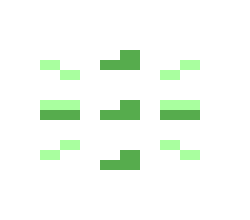
\includegraphics[height=1.2cm]{src/meanie_explosion_sprites/3_MEANIE_EXPLOSION_2.png}}
\hspace{1.0cm}
\raisebox{-0.2\totalheight}{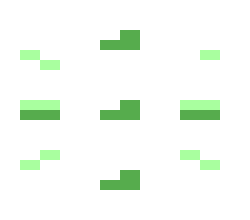
\includegraphics[height=1.2cm]{src/meanie_explosion_sprites/3_MEANIE_EXPLOSION_3.png}}
\hspace{1.0cm}
\raisebox{-0.2\totalheight}{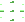
\includegraphics[height=1.2cm]{src/meanie_explosion_sprites/3_MEANIE_EXPLOSION_4.png}}
\hspace{1.0cm}
\raisebox{-0.2\totalheight}{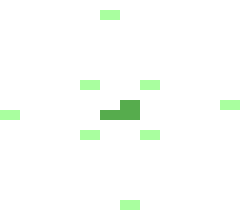
\includegraphics[height=1.2cm]{src/meanie_explosion_sprites/3_MEANIE_EXPLOSION_5.png}}
\hspace{1.0cm}

But it turns out this blast is followed by a secondary explosion which is subtly different. There is less
meanie material fuelling this phase of the detonation so it is slightly lighter, with fewer blast fragments at
its centre.

\hspace{0.5cm}
\raisebox{-0.2\totalheight}{
\includegraphics[height=1.2cm]{src/meanie_explosion_sprites/3_MEANIE_SECONDARY_1.png}}
\hspace{1.0cm}
\raisebox{-0.2\totalheight}{
\includegraphics[height=1.2cm]{src/meanie_explosion_sprites/3_MEANIE_SECONDARY_2.png}}
\hspace{1.0cm}
\raisebox{-0.2\totalheight}{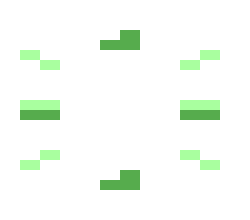
\includegraphics[height=1.2cm]{src/meanie_explosion_sprites/3_MEANIE_SECONDARY_3.png}}
\hspace{1.0cm}
\raisebox{-0.2\totalheight}{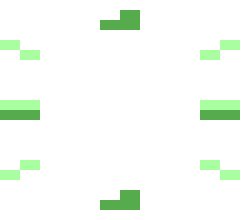
\includegraphics[height=1.2cm]{src/meanie_explosion_sprites/3_MEANIE_SECONDARY_4.png}}
\hspace{1.0cm}
\raisebox{-0.2\totalheight}{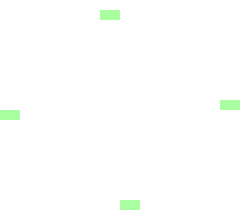
\includegraphics[height=1.2cm]{src/meanie_explosion_sprites/3_MEANIE_SECONDARY_5.png}}
\hspace{1.0cm}

So the complete effect of an exploding enemy consists of 10 sprites in total. A surprising number, but consistent
with the detail devoted to other effects in the game such as the manta's manouevres. Even though the explosion
sprites are sparse they are not devoid of detail. We get a sense of the care devoted to their colour gradations
when we blow them up into diagrams illustrating the full blast sequence.
\clearpage

\begin{figure}[H]
    \centering
    \begin{adjustbox}{width=14.2cm,center}
      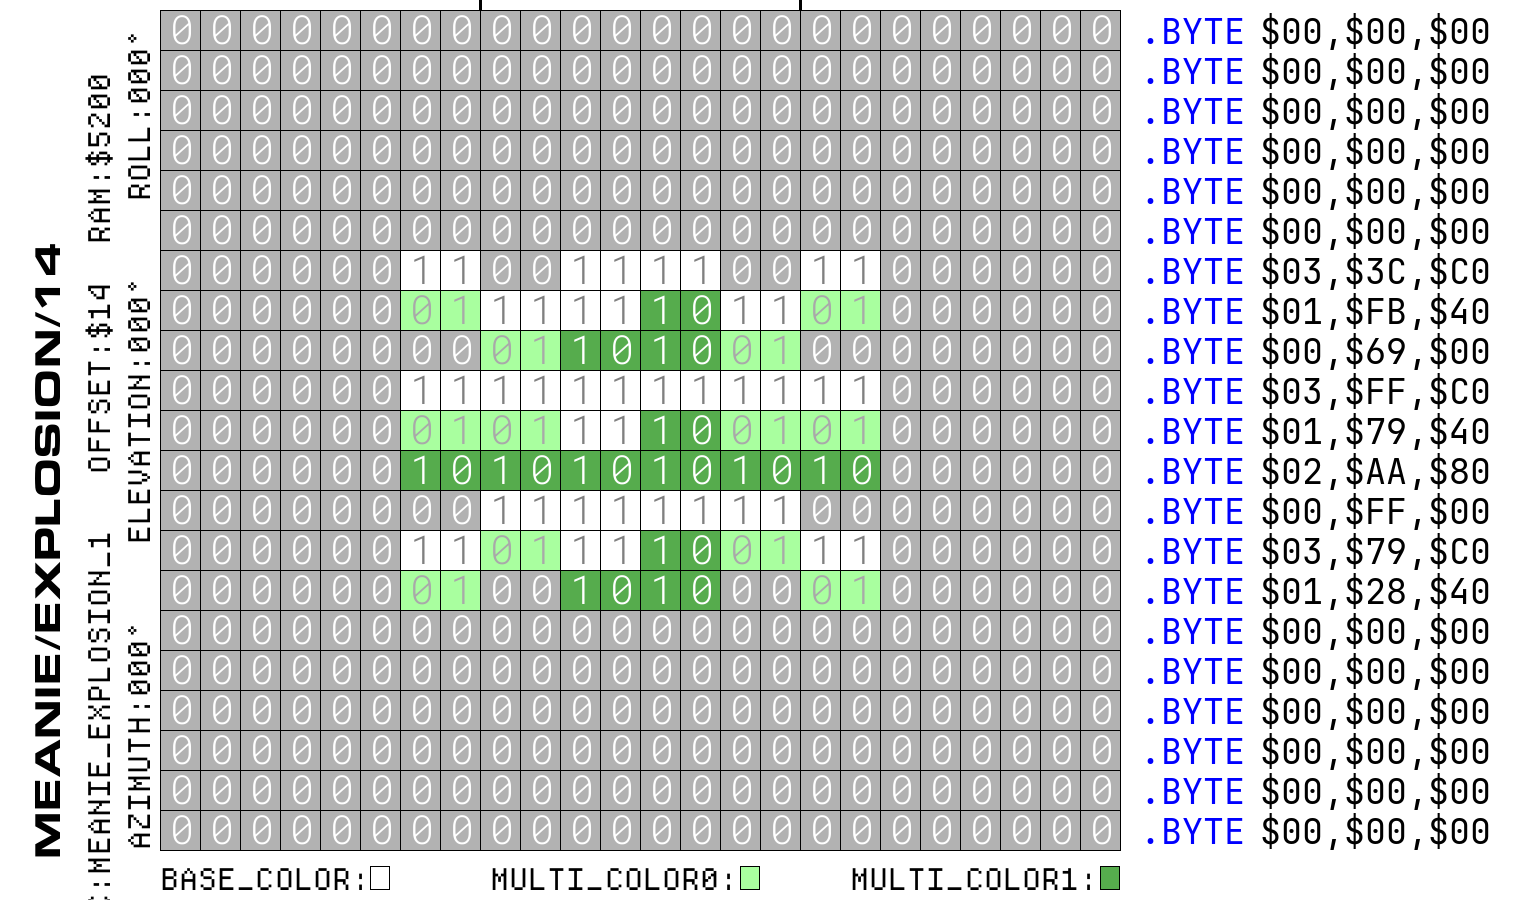
\includegraphics[width=7cm]{src/meanie_explosion_diagrams_list/3_MEANIE_8.png}%
      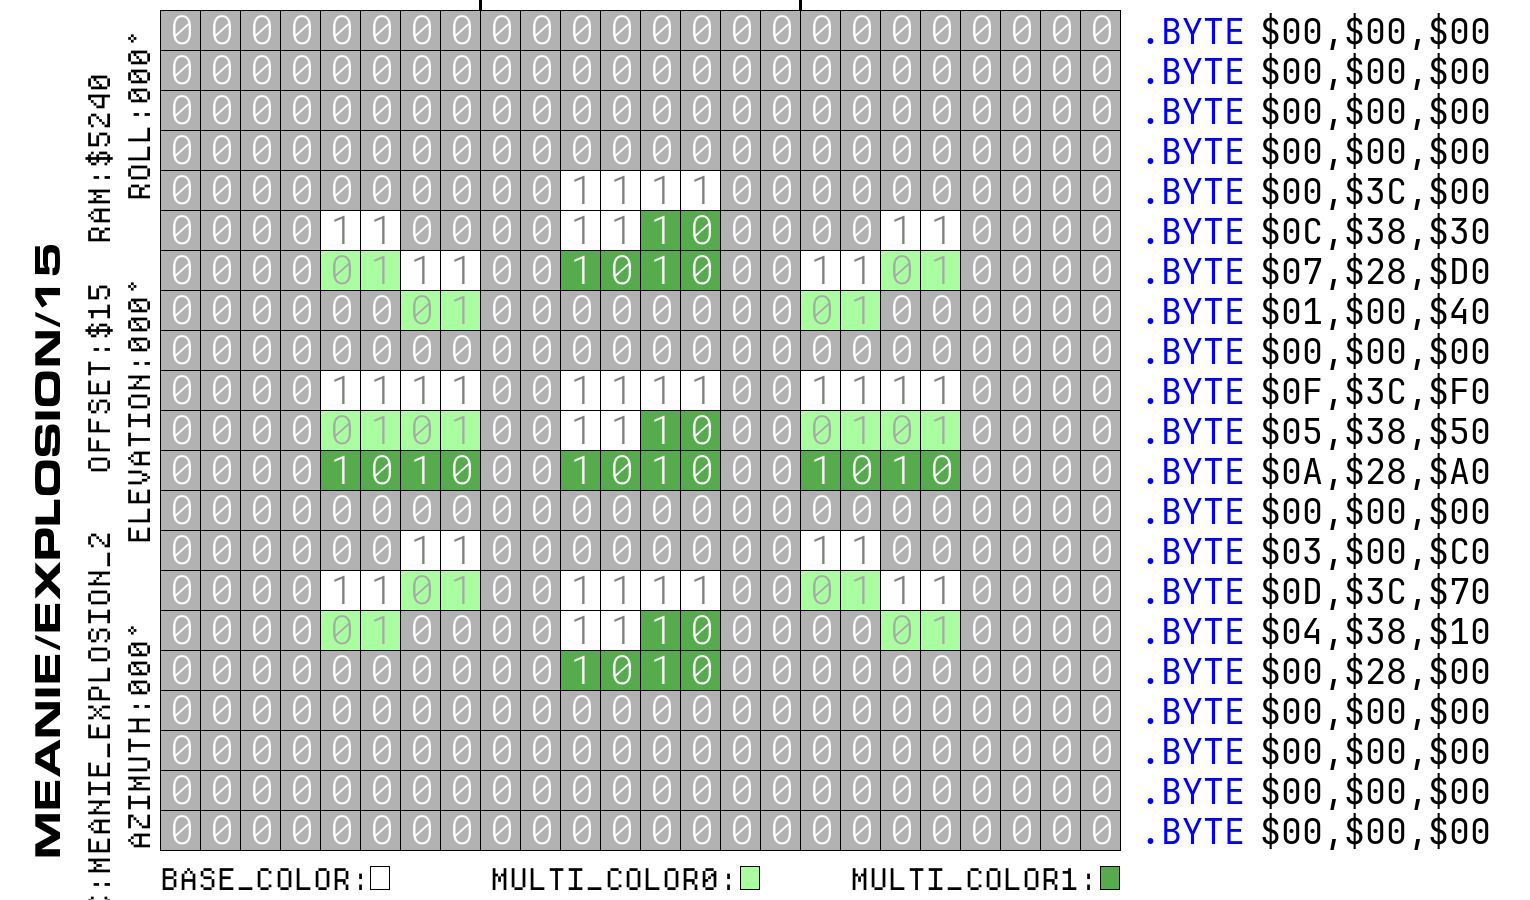
\includegraphics[width=7cm]{src/meanie_explosion_diagrams_list/3_MEANIE_9.png}%
    \end{adjustbox}
\end{figure}
\vspace{-0.5cm}
\begin{figure}[H]
    \centering
    \begin{adjustbox}{width=14.2cm,center}
      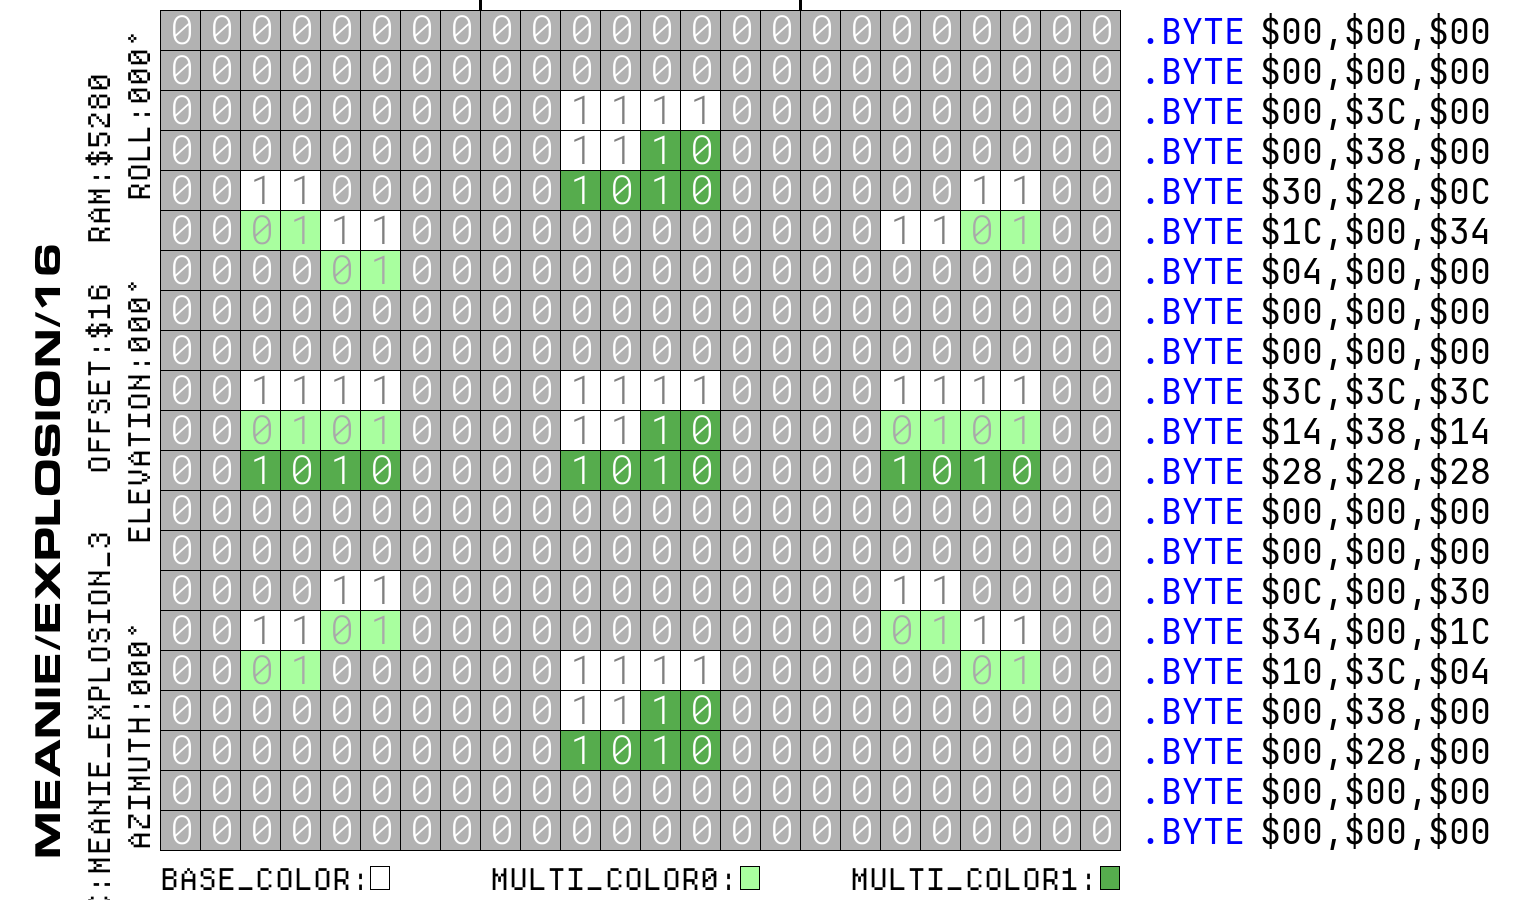
\includegraphics[width=7cm]{src/meanie_explosion_diagrams_list/3_MEANIE_10.png}%
      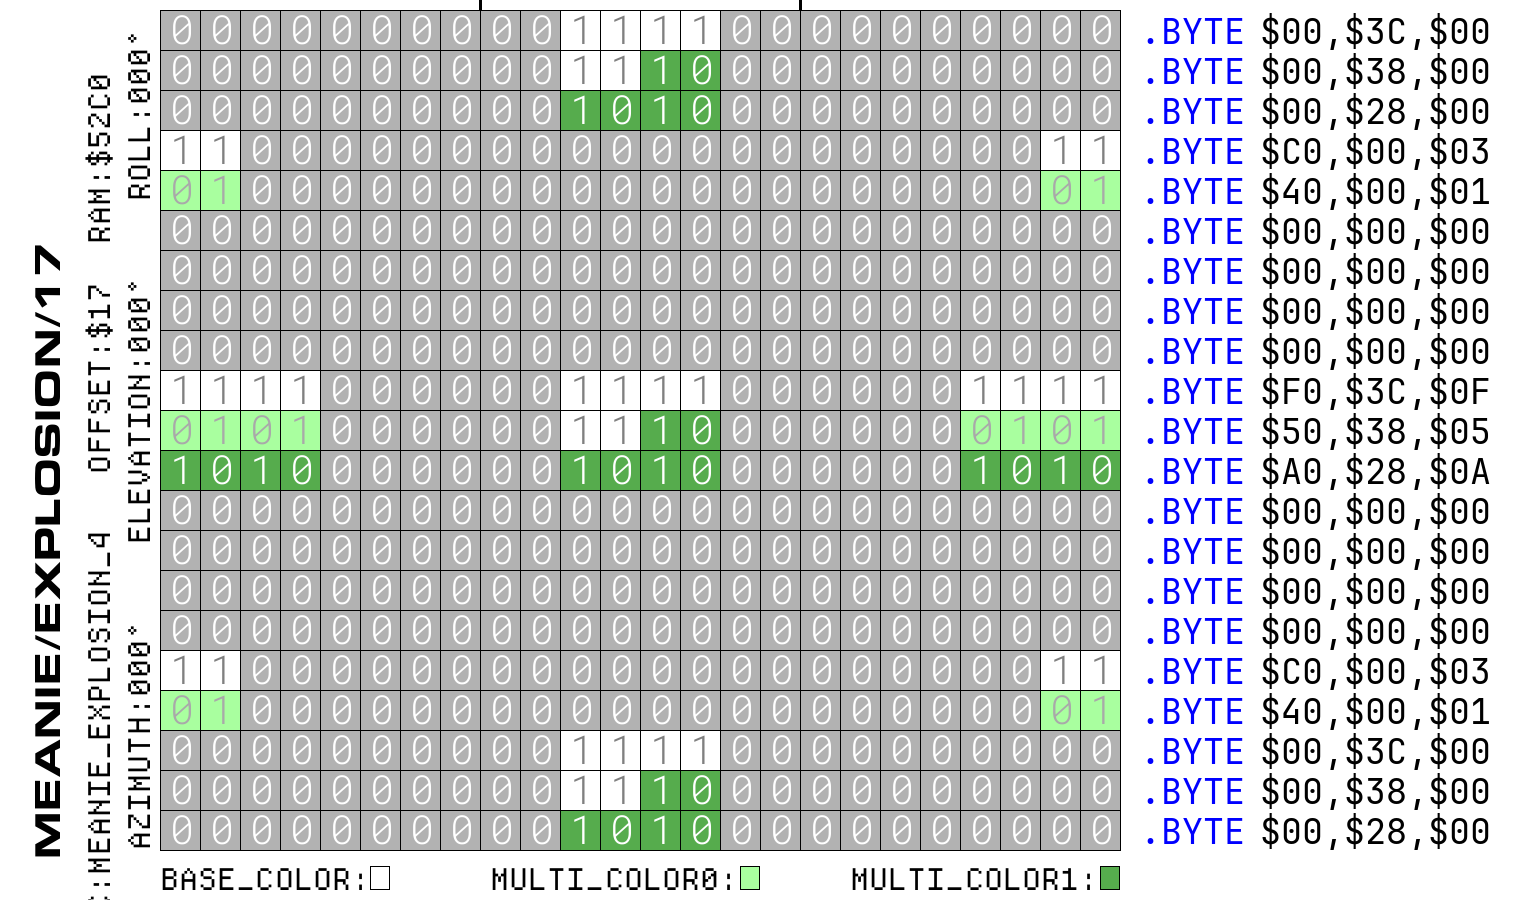
\includegraphics[width=7cm]{src/meanie_explosion_diagrams_list/3_MEANIE_11.png}%
    \end{adjustbox}
\end{figure}
\vspace{-0.5cm}
\begin{figure}[H]
    \centering
    \begin{adjustbox}{width=14.2cm,center}
      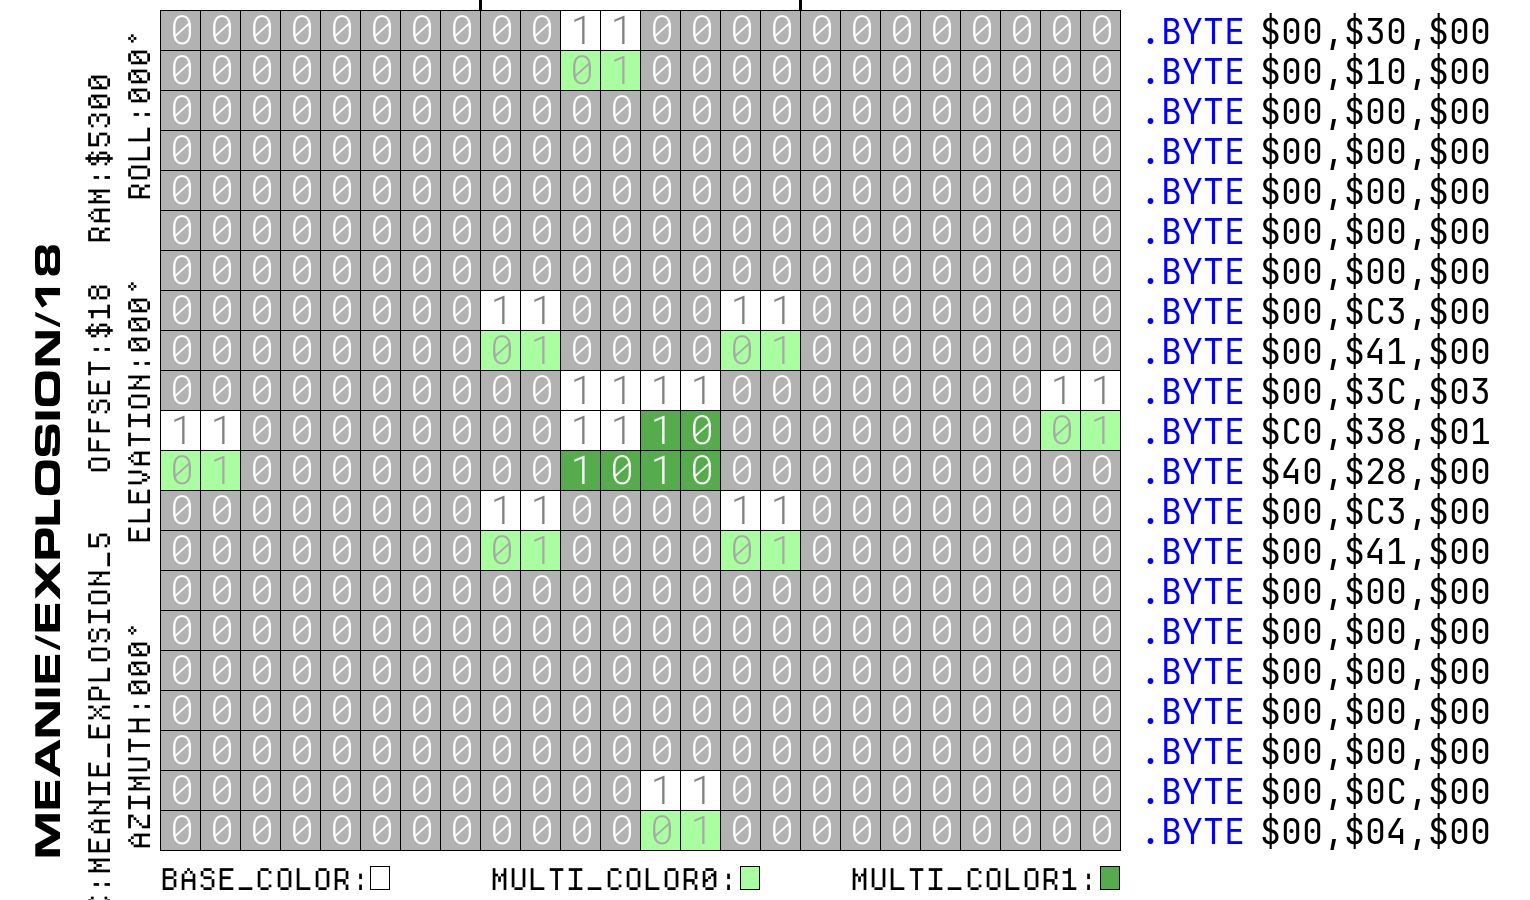
\includegraphics[width=7cm]{src/meanie_explosion_diagrams_list/3_MEANIE_12.png}%
      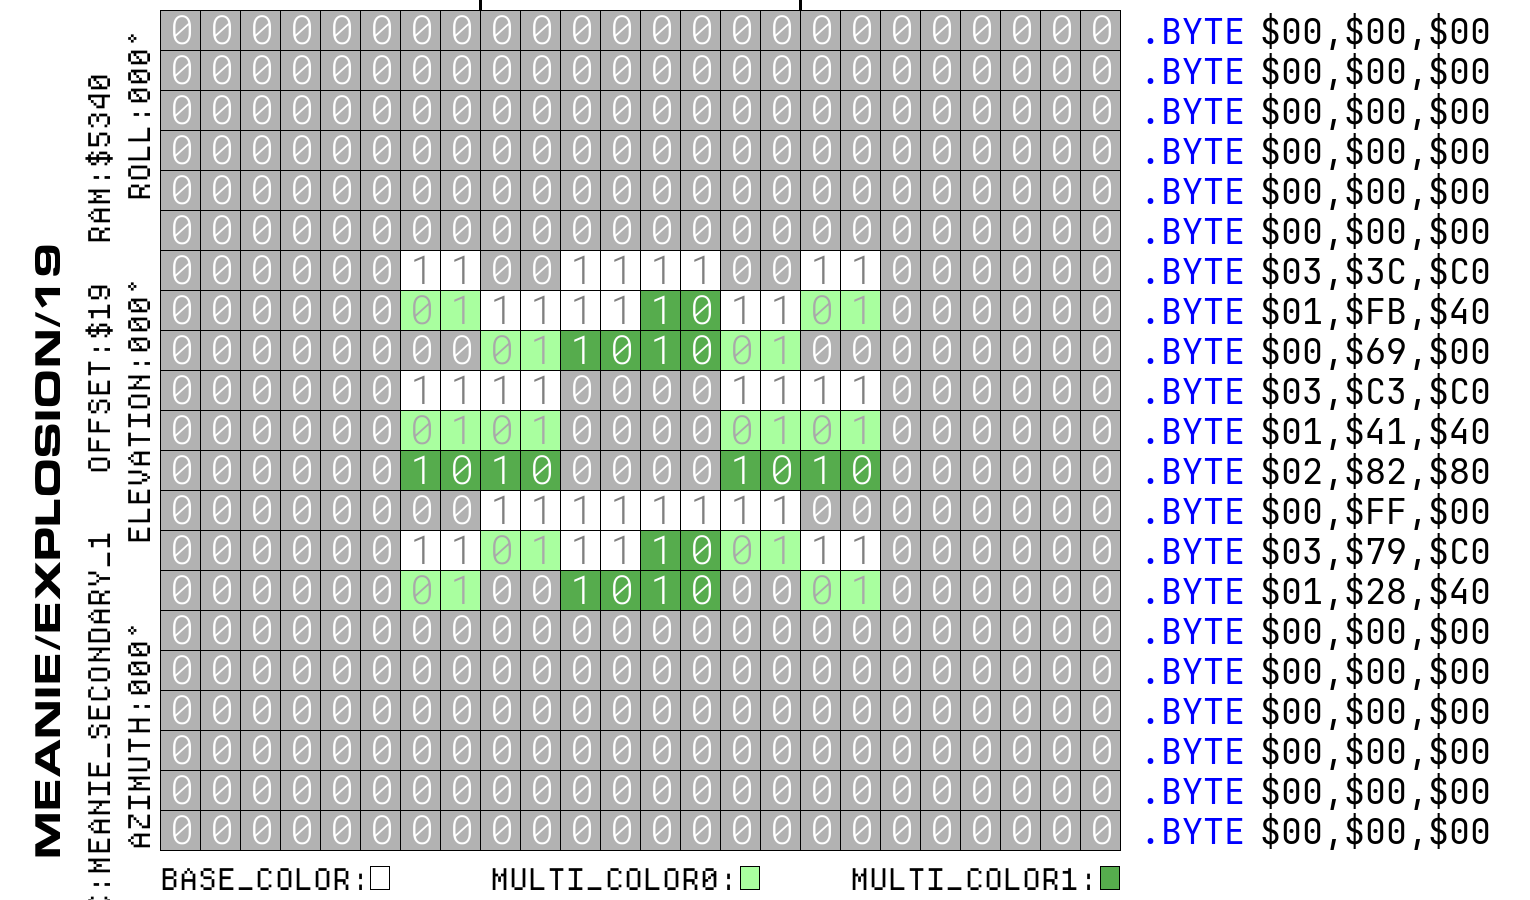
\includegraphics[width=7cm]{src/meanie_explosion_diagrams_list/3_MEANIE_13.png}%
    \end{adjustbox}
\end{figure}
\vspace{-0.5cm}
\begin{figure}[H]
    \centering
    \begin{adjustbox}{width=14.2cm,center}
      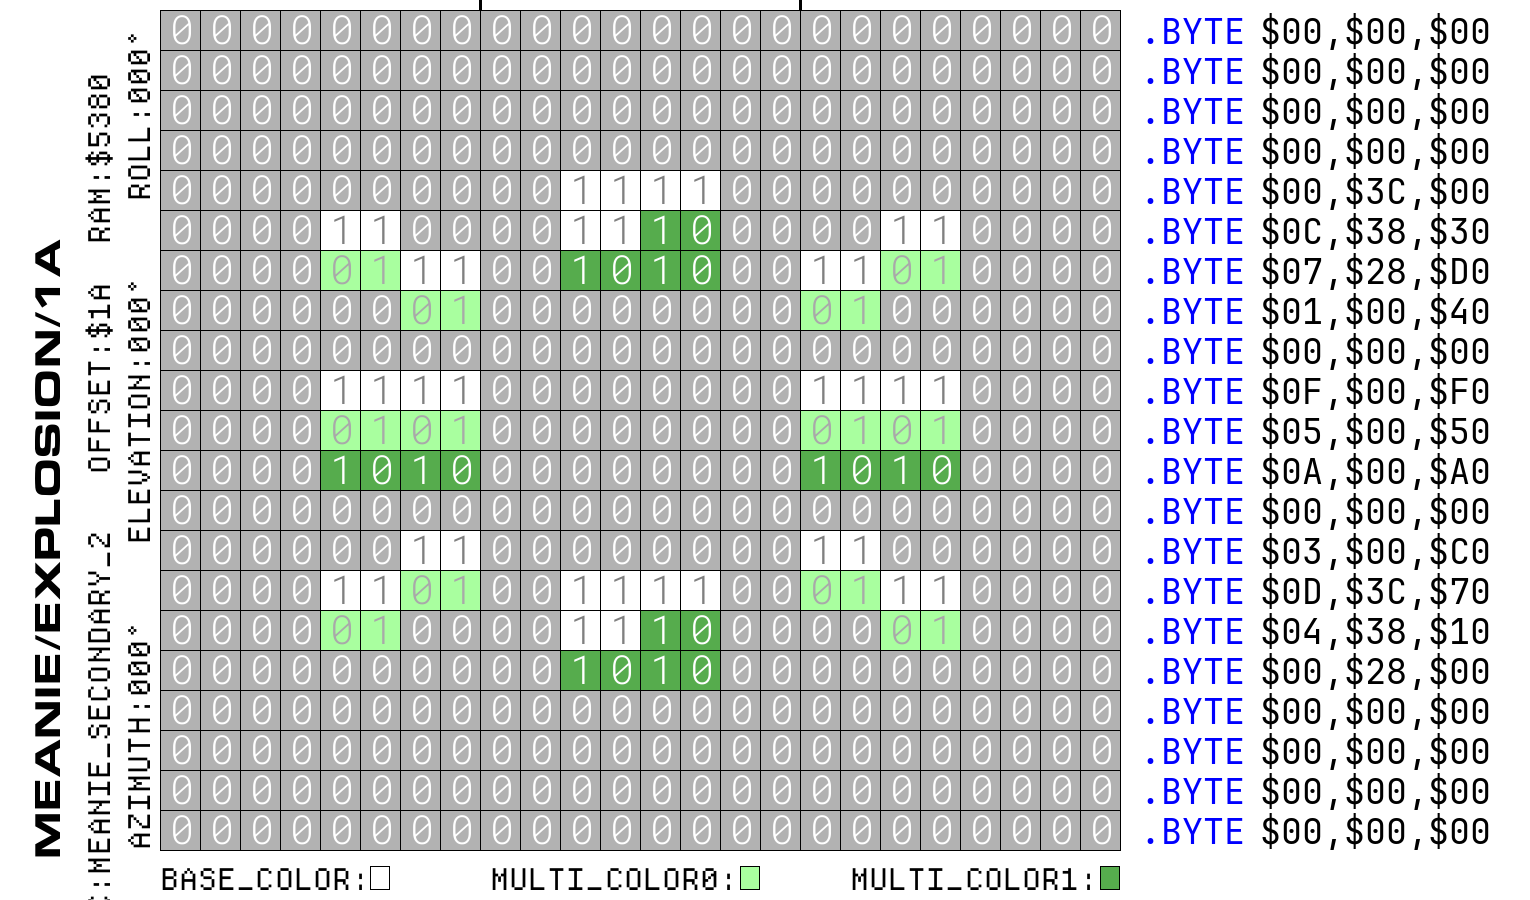
\includegraphics[width=7cm]{src/meanie_explosion_diagrams_list/3_MEANIE_14.png}%
      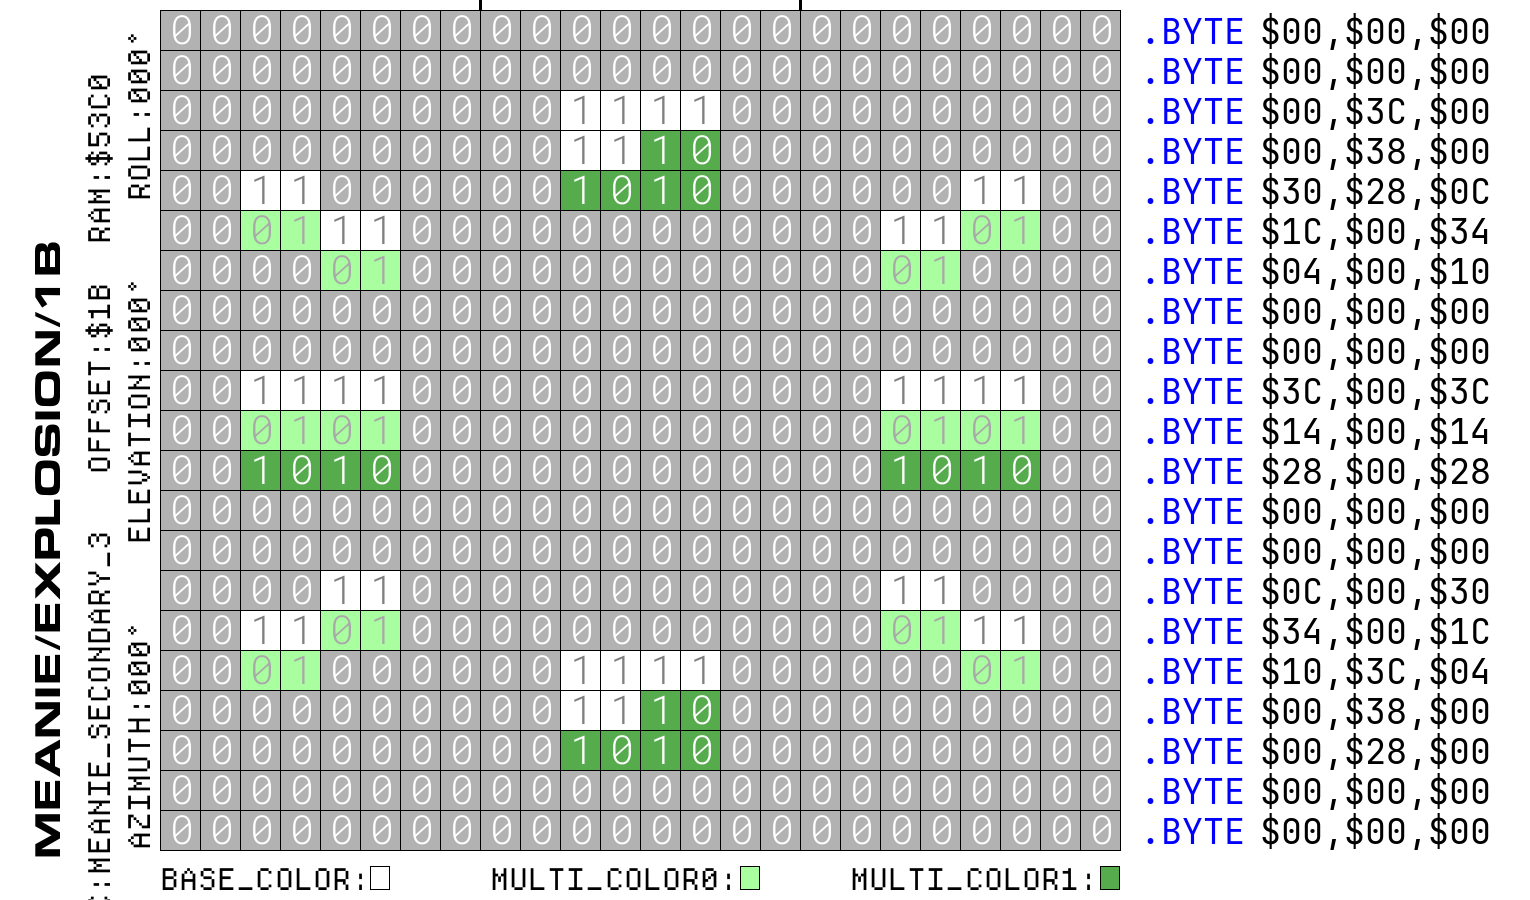
\includegraphics[width=7cm]{src/meanie_explosion_diagrams_list/3_MEANIE_15.png}%
    \end{adjustbox}
\end{figure}
\vspace{-0.5cm}
\begin{figure}[H]
    \centering
    \begin{adjustbox}{width=14.2cm,center}
      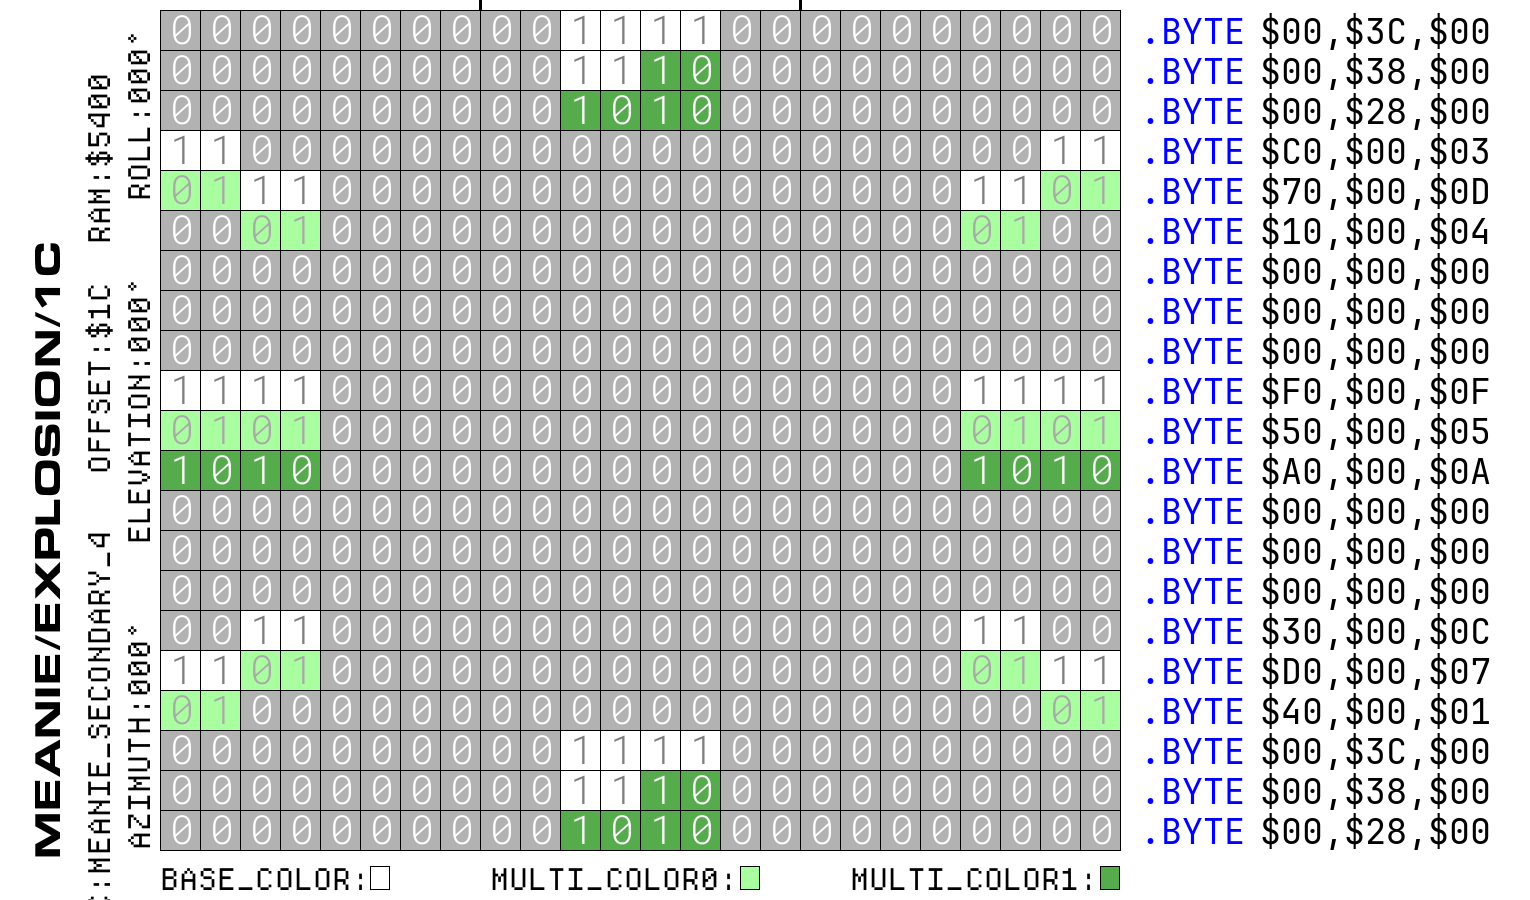
\includegraphics[width=7cm]{src/meanie_explosion_diagrams_list/3_MEANIE_16.png}%
      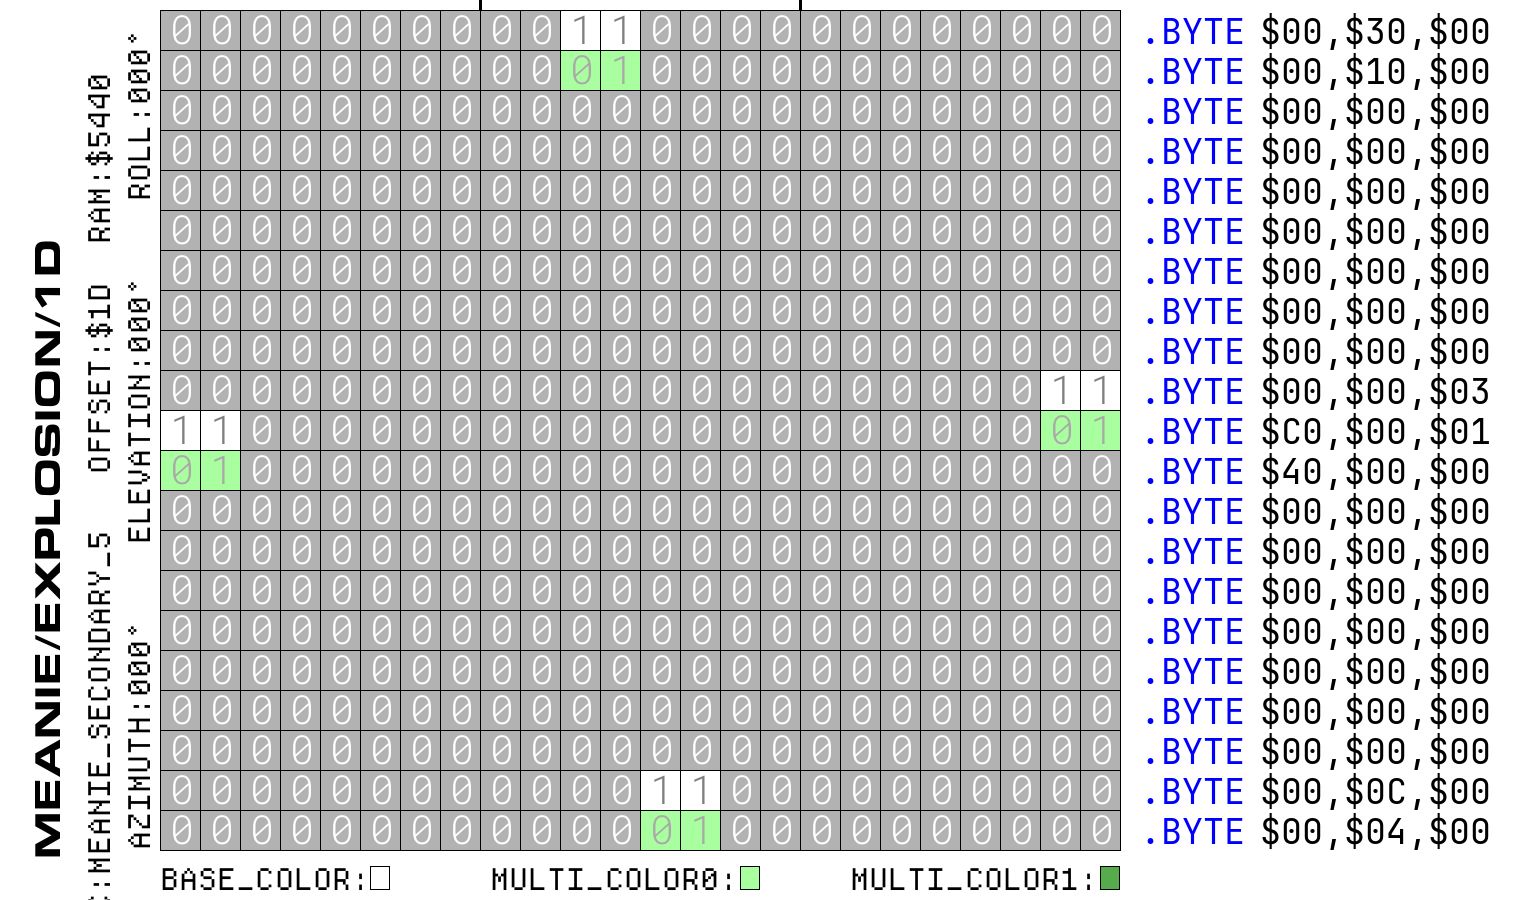
\includegraphics[width=7cm]{src/meanie_explosion_diagrams_list/3_MEANIE_17.png}%
    \end{adjustbox}
\end{figure}

There is the usual detail to sort out when managing an incident of this sort. The routine
below first has to deal with restoring the surface under the player bullet (now that
it has disappeared after striking an enemy), it has to decide whether to award a score to
the player, and then
finally it must set the explosion in train. The two main elements of this last task are to 
designate the new 'active' function for the meanie (to the self-explanatory
\fcode{AnimateEnemyExplosion}) and to specify the new sprite for the
meanie, which in this case will be the first frame of the explosion sequence, sprite \icode{\$14}
which we can see on the top left of the opposite page.

\begin{lstlisting}[basicstyle=\scriptsize\ttfamily, escapechar=\%]
EnemyShipWasHit
  LDA playerBulletSlotArray,X        ; Get the bullet that struck the meanie.
  BEQ MaybeAwardScore                ; Skip to score check, if no bullet.
  ; Restore any dreadnought surface underneath the removed bullet.
  LDA playerBulletRamLoPtrArray,X    ; Get Lo Ptr to surface under bullet.
  STA screenRAMLoPtr                 ; Store it.
  LDA playerBulletRamHiPtrArray,X    ; Get Hi Ptr to surface under bullet.
  STA screenRAMHiPtr                 ; Store it.
  LDY #$00                           ; Store 0 in Y index.
  LDA charBehindPlayerBulletArray,X  ; Get the character under the bullet.
  STA (screenRAMLoPtr),Y             ; Restore it to the surface.
  LDA #$00                           ; Clear the bullet that struck the meanie..
  STA playerBulletSlotArray,X        ; .. from the bullet tracking array.

MaybeAwardScore   
  LDA meanieEarnsPoints              ; Get whether the meanie earns points.
  BNE InitiateMeanieExplosion        ; If not, go ahead and explode it.
  LDY scoreToAddForHittingEnemy      ; Get the score for the meanie.
  JSR AddScoresFromHittingStuff      ; Add it to the player's score.

InitiateMeanieExplosion
  LDA #$26                           ; Get the explosion sound.
  STA soundToPlay                    ; Store it for playing later.
  LDY enemyIndex                     ; Get the index for the meanie.
  ; The routine AnimateEnemyExplosion will manage the explosion animation,
  ; so we set it here as the 'active' function for the meanie.
  LDA #$06                           ; Get the index to AnimateEnemyExplosion
  STA indexToEnemyUpdatePtrArray,Y   ; Set it as the meanie's active function.
  ; Set the explosion in train by selecting its initial sprite.
  LDA #$14                           ; Explosion's starting sprite: %\raisebox{-0.2\totalheight}{
\includegraphics[height=0.30cm]{src/meanie_explosion_sprites/3_MEANIE_EXPLOSION_1.png}}% 
  STA currentSpriteValue             ; Store it as the meanie's new sprite.
  DEC numberOfEnemiesSpawned         ; Decrement the enemy count.
  JMP UpdateEnemyContentAndPosition  ; Display our updates to the meanie.
\end{lstlisting}

The routine we have now designated for governing the sprite's behaviour, \fcode{Animate\-EnemyExplosion},
takes care of the relatively simple task of incrementing the sprite value for the meanie from \icode{\$14}
all the way up to \icode{\$1D}. It does this by incrementing it using a rate limiter to control the
pace at which the blast happens. Notice that it also ensures the exploding enemy continues to gravitate
towards the enemy along the horizontal position. This is a small but important detail for reinforcing the
versimilitude of the explosion: the enemy may be destroyed but its inertial movement drives it inexorably
towards its adversary.

\begin{lstlisting}[basicstyle=\scriptsize\ttfamily, escapechar=\%]
AnimateEnemyExplosion
  JSR UpdateSpriteXPosToFollowManta  ; Keep the explosion moving towards the manta.
  LDA frameRate                      ; Check our update rate limiter.
  AND #$01                           ; We only update every second visit.
  BNE NoFurtherActionRequired        ; Skip update if rate limit says so.
  ; Move to the next frame in the explosion sequence.
  INC currentSpriteValue             ; Increment the sprite value.
  LDA currentSpriteValue             ; Load it to the A register.
  CMP #$1E                           ; Have we reached the final sprite: %\raisebox{-0.2\totalheight}{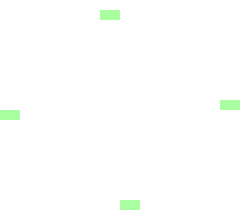
\includegraphics[height=0.30cm]{src/meanie_explosion_sprites/3_MEANIE_SECONDARY_5.png}}% ?
  BCC NoFurtherActionRequired        ; If not, we're done for now.
  ; Otherwise the explosion is over, so clean up.
  LDA #$00                           ; Load 0 to the A register.
  STA currentSpriteEnabled     ; Use it to turn the sprite 'off'.
  LDY numberOfEnemiesToUpdate        ; Get the meanie's index.
  STA indexToEnemyUpdatePtrArray,Y   ; Make it's active function 'DoNothing'.
  DEC shouldWeLaunchMine             ; Dead enemies factor into mine launch decisions.
  JSR DisplayCurrentSprite           ; Update the meanie so that it disappears.
  RTS

NoFurtherActionRequired
  JMP DetectSpriteLeavingScreen      ; Check if the sprite has left the screen.
\end{lstlisting}

By comparison the manta's explosion seems almost banal. There is no secondary phase, just a fulsome puff of fire.
But to judge the quality of the blast on the sprites alone would be a mistake. There is a lot more going on than
meets the eye in a mere enumeration of the sprites.

\raisebox{-0.2\totalheight}{
\includegraphics[height=1.2cm]{src/manta_explosion_sprites/1_EXPLOSION_MAJOR1.png}}
\hspace{1.0cm}
\raisebox{-0.2\totalheight}{
\includegraphics[height=1.2cm]{src/manta_explosion_sprites/1_EXPLOSION_MAJOR2.png}}
\hspace{1.0cm}
\raisebox{-0.2\totalheight}{
\includegraphics[height=1.2cm]{src/manta_explosion_sprites/1_EXPLOSION_MAJOR3.png}}
\hspace{1.0cm}
\raisebox{-0.2\totalheight}{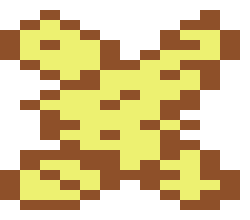
\includegraphics[height=1.2cm]{src/manta_explosion_sprites/1_EXPLOSION_MAJOR4.png}}
\hspace{1.0cm}
\raisebox{-0.2\totalheight}{
\includegraphics[height=1.2cm]{src/manta_explosion_sprites/1_EXPLOSION_MAJOR5.png}}
\hspace{1.0cm}
\raisebox{-0.2\totalheight}{
\includegraphics[height=1.2cm]{src/manta_explosion_sprites/1_EXPLOSION_MAJOR6.png}}
\hspace{1.0cm}

\hspace{0.8cm}
\raisebox{-0.2\totalheight}{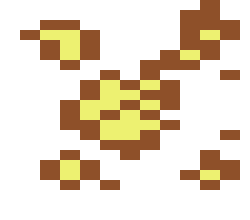
\includegraphics[height=1.2cm]{src/manta_explosion_sprites/1_EXPLOSION_MAJOR7.png}}
\hspace{1.0cm}
\raisebox{-0.2\totalheight}{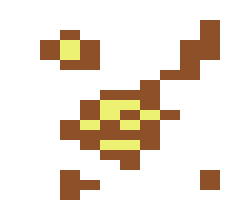
\includegraphics[height=1.2cm]{src/manta_explosion_sprites/1_EXPLOSION_MAJOR8.png}}
\hspace{1.0cm}
\raisebox{-0.2\totalheight}{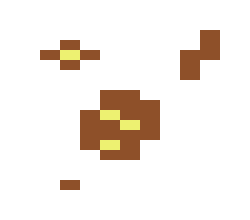
\includegraphics[height=1.2cm]{src/manta_explosion_sprites/1_EXPLOSION_MAJOR9.png}}
\hspace{1.0cm}
\raisebox{-0.2\totalheight}{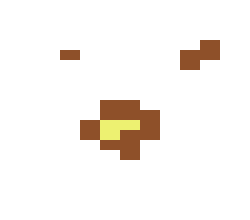
\includegraphics[height=1.2cm]{src/manta_explosion_sprites/1_EXPLOSION_MAJOR10.png}}
\hspace{1.0cm}
\raisebox{-0.2\totalheight}{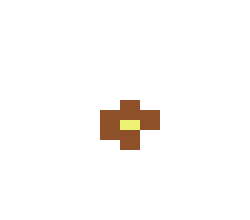
\includegraphics[height=1.2cm]{src/manta_explosion_sprites/1_EXPLOSION_MAJOR11.png}}
\hspace{1.0cm}

Even though the sprites used for the manta's explosion are beefier than the those used for the enemy sprites and
even though a full eleven are dedicated to a single detonation, it might still be considered weak sauce if that
was all that we rendered when the manta blows up. So not only do we create a secondary detonation for the explosion
we go much further and generate eight separate explosions that run in lock step with each other and are composited
together to create a satisfying, churning blast that roils on the surface of the dreadnought. 

As always it is easier to visualize this effect than describe it, so below we show in practice what this means.
On the left we have eight separate explosion sequences, each running in parallel but at slightly different stages
of detonation. Those to the left of the picture are further advanced than those to the right. You will notice that each blast
has been dithered at random from it's centre along both the horizontal and vertical axis. On the right hand side we
see the result of compositing all eight of these explosions together. To any player of \textit{Uridium} this will look 
more familiar: the manta's explosion is all eight explosions rolled together into a pulsing ball of fire.


\begin{figure}[H]
    \centering
    \begin{adjustbox}{center}
      \hspace{0.5cm}
      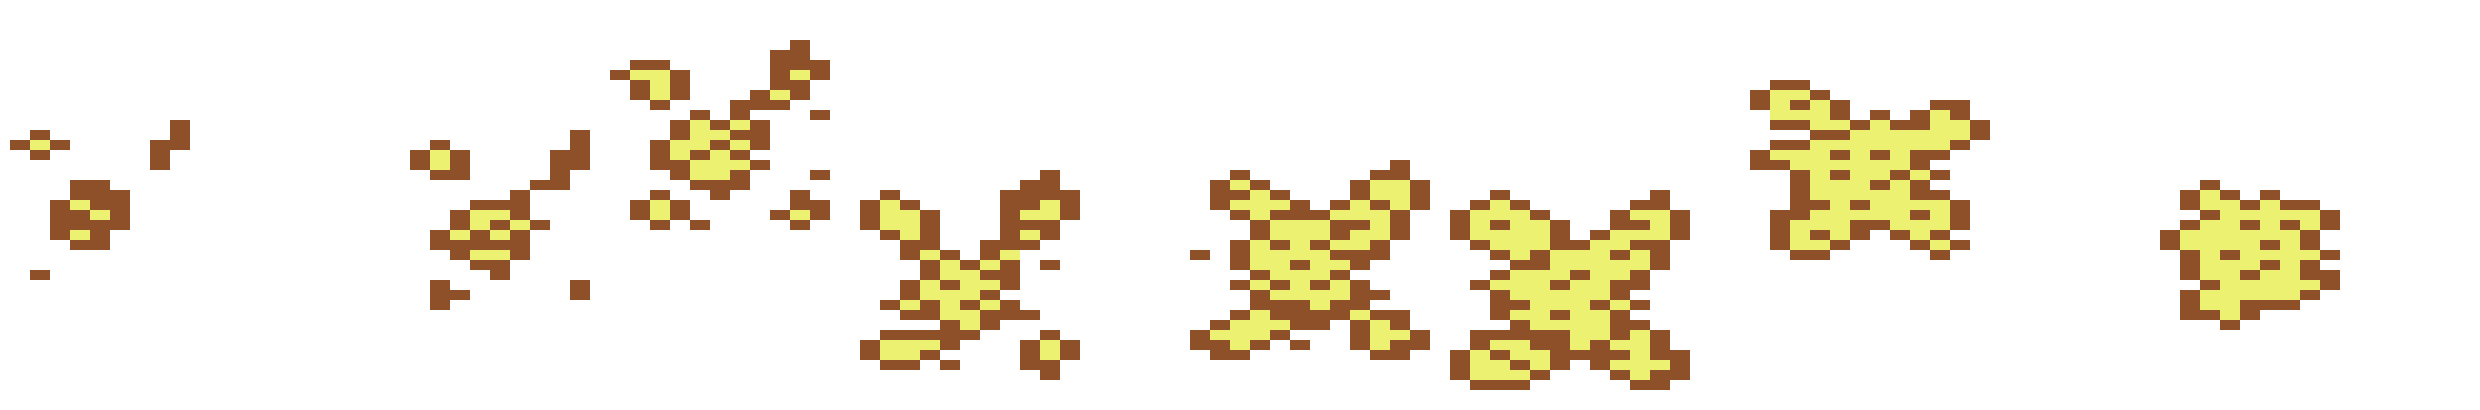
\includegraphics[height=1.6cm]{src/manta_explosion_sprites/sidebyside_explosion_9.png}%
      \hspace{0.5cm}
      \raisebox{1.2\totalheight}{
\includegraphics[height=0.4cm]{src/baydoor_sprites/arrow.png}}
      \hspace{0.3cm}
      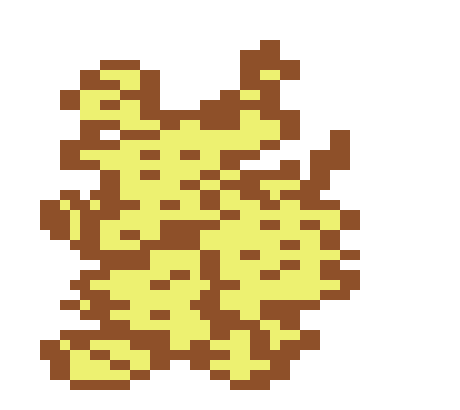
\includegraphics[height=1.6cm]{src/manta_explosion_sprites/composite_explosion_9.png}%
    \end{adjustbox}
\end{figure}
\vspace{-0.4cm}

Running all these together from beginning to end takes only 21 frames or so. We can watch the progress from beginning
to end of the fireball over just a couple of pages.
As the sequence gets up and running we notice that it starts with just one member but with each frame
that we advance a new member is added until all 8 slots are filled.

\begin{figure}[H]
    \centering
    \begin{adjustbox}{center}
      \hspace{0.5cm}
      
\includegraphics[height=1.6cm]{src/manta_explosion_sprites/sidebyside_explosion_1.png}%
      \hspace{0.5cm}
      \raisebox{1.2\totalheight}{
\includegraphics[height=0.4cm]{src/baydoor_sprites/arrow.png}}
      \hspace{0.3cm}
      
\includegraphics[height=1.6cm]{src/manta_explosion_sprites/composite_explosion_1.png}%
    \end{adjustbox}
\end{figure}
\vspace{-0.4cm}
\begin{figure}[H]
    \centering
    \begin{adjustbox}{center}
      \hspace{0.5cm}
      
\includegraphics[height=1.6cm]{src/manta_explosion_sprites/sidebyside_explosion_2.png}%
      \hspace{0.5cm}
      \raisebox{1.2\totalheight}{
\includegraphics[height=0.4cm]{src/baydoor_sprites/arrow.png}}
      \hspace{0.3cm}
      
\includegraphics[height=1.6cm]{src/manta_explosion_sprites/composite_explosion_2.png}%
    \end{adjustbox}
\end{figure}
\vspace{-0.4cm}
\begin{figure}[H]
    \centering
    \begin{adjustbox}{center}
      \hspace{0.5cm}
      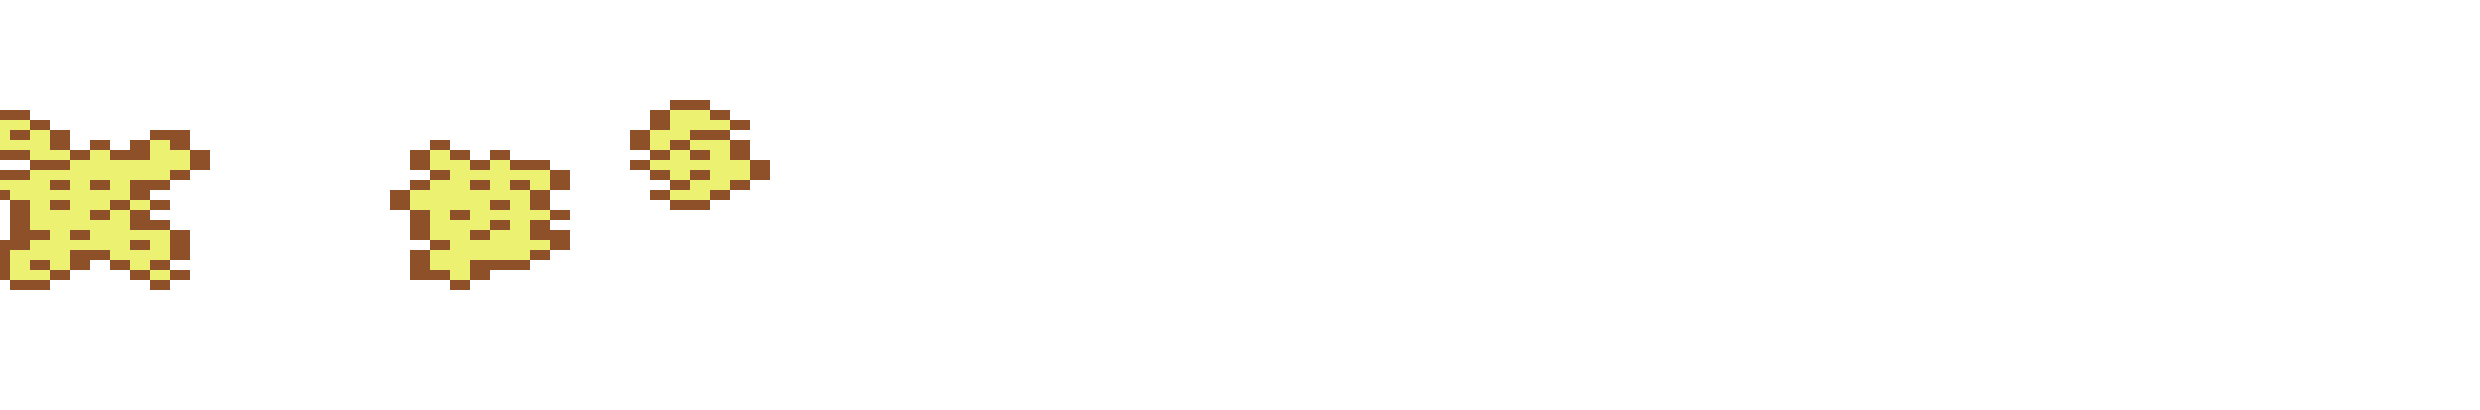
\includegraphics[height=1.6cm]{src/manta_explosion_sprites/sidebyside_explosion_3.png}%
      \hspace{0.5cm}
      \raisebox{1.2\totalheight}{
\includegraphics[height=0.4cm]{src/baydoor_sprites/arrow.png}}
      \hspace{0.3cm}
      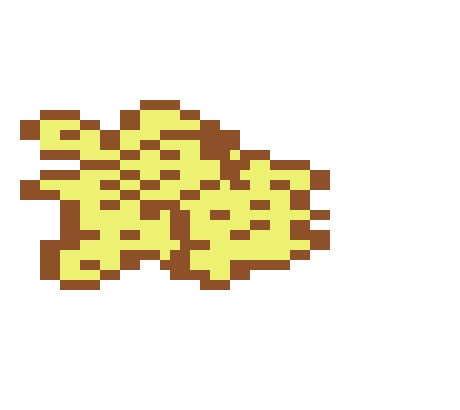
\includegraphics[height=1.6cm]{src/manta_explosion_sprites/composite_explosion_3.png}%
    \end{adjustbox}
\end{figure}
\vspace{-0.4cm}
\begin{figure}[H]
    \centering
    \begin{adjustbox}{center}
      \hspace{0.5cm}
      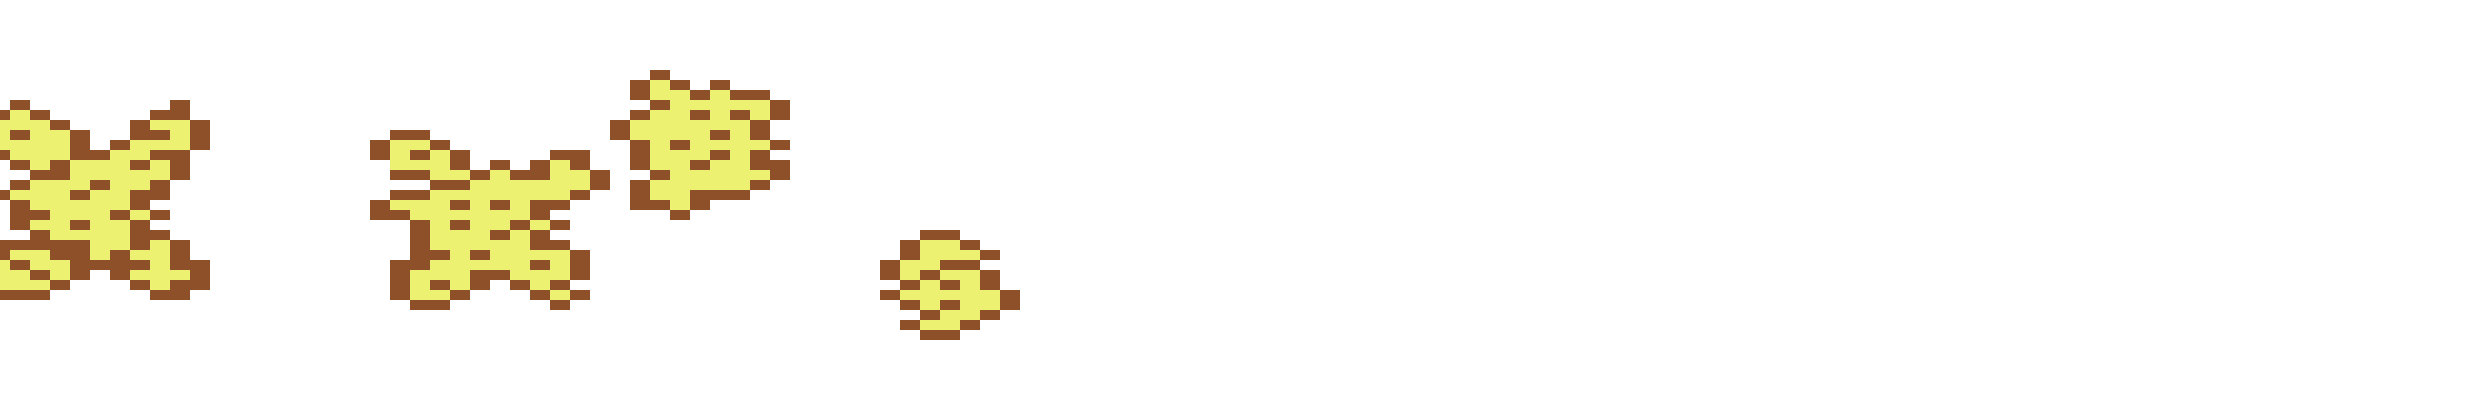
\includegraphics[height=1.6cm]{src/manta_explosion_sprites/sidebyside_explosion_4.png}%
      \hspace{0.5cm}
      \raisebox{1.2\totalheight}{
\includegraphics[height=0.4cm]{src/baydoor_sprites/arrow.png}}
      \hspace{0.3cm}
      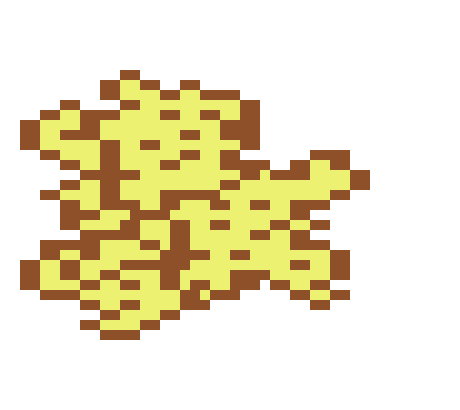
\includegraphics[height=1.6cm]{src/manta_explosion_sprites/composite_explosion_4.png}%
    \end{adjustbox}
\end{figure}
\vspace{-0.4cm}
\begin{figure}[H]
    \centering
    \begin{adjustbox}{center}
      \hspace{0.5cm}
      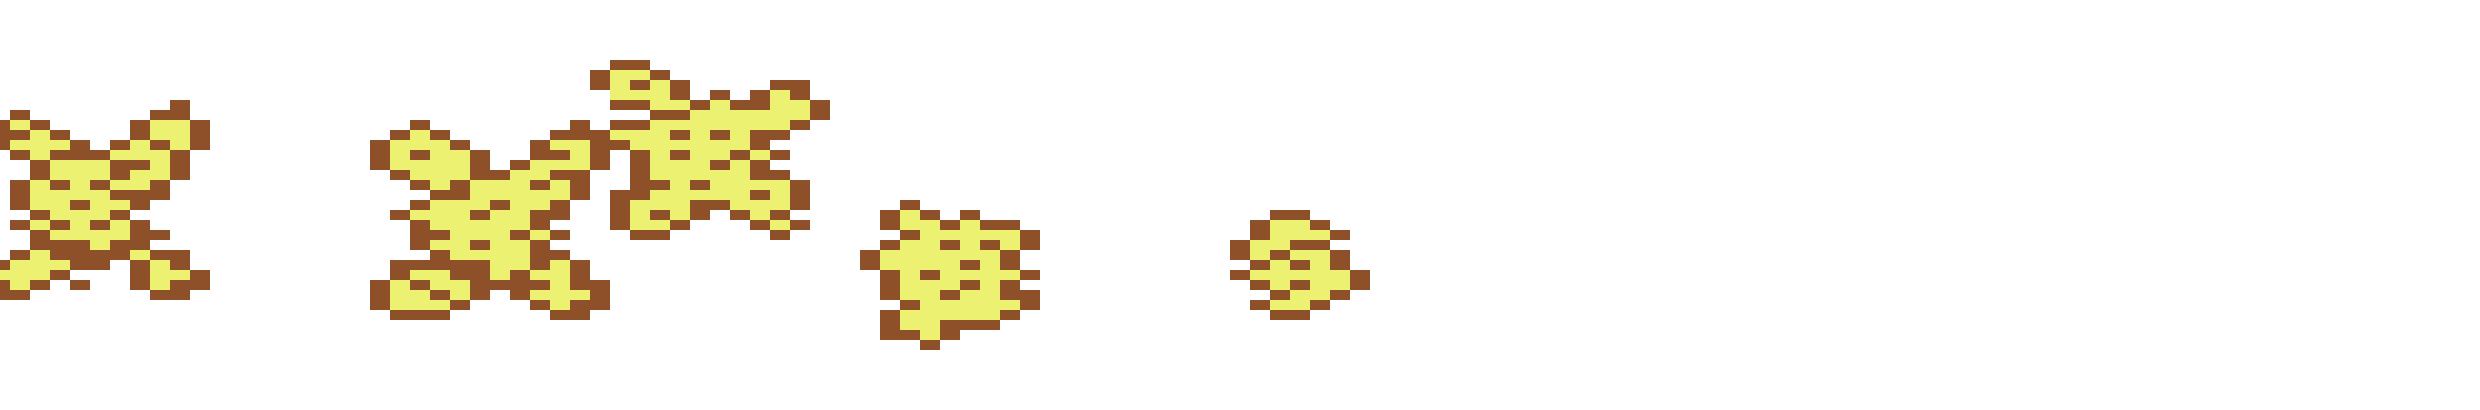
\includegraphics[height=1.6cm]{src/manta_explosion_sprites/sidebyside_explosion_5.png}%
      \hspace{0.5cm}
      \raisebox{1.2\totalheight}{
\includegraphics[height=0.4cm]{src/baydoor_sprites/arrow.png}}
      \hspace{0.3cm}
      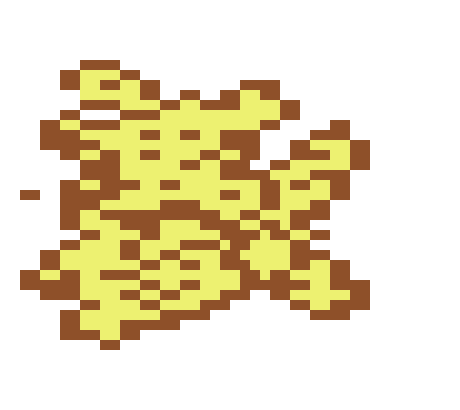
\includegraphics[height=1.6cm]{src/manta_explosion_sprites/composite_explosion_5.png}%
    \end{adjustbox}
\end{figure}
\vspace{-0.4cm}
\begin{figure}[H]
    \centering
    \begin{adjustbox}{center}
      \hspace{0.5cm}
      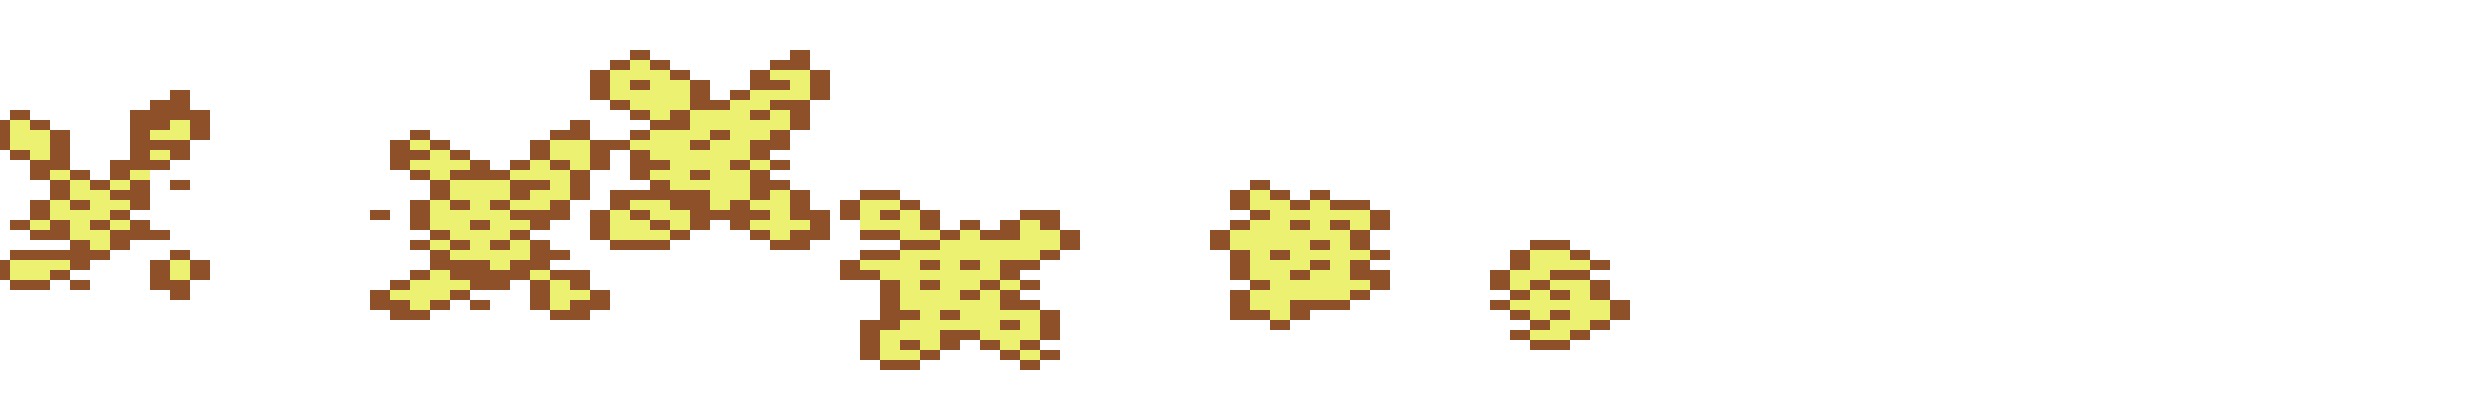
\includegraphics[height=1.6cm]{src/manta_explosion_sprites/sidebyside_explosion_6.png}%
      \hspace{0.5cm}
      \raisebox{1.2\totalheight}{
\includegraphics[height=0.4cm]{src/baydoor_sprites/arrow.png}}
      \hspace{0.3cm}
      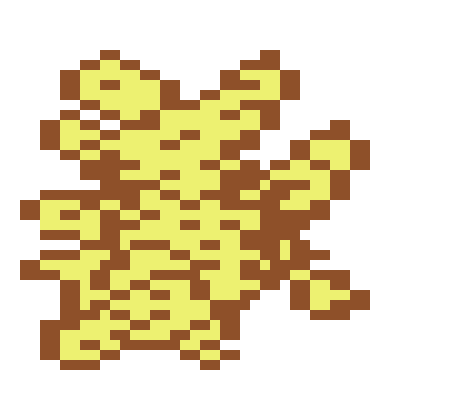
\includegraphics[height=1.6cm]{src/manta_explosion_sprites/composite_explosion_6.png}%
    \end{adjustbox}
\end{figure}
\vspace{-0.4cm}
\begin{figure}[H]
    \centering
    \begin{adjustbox}{center}
      \hspace{0.5cm}
      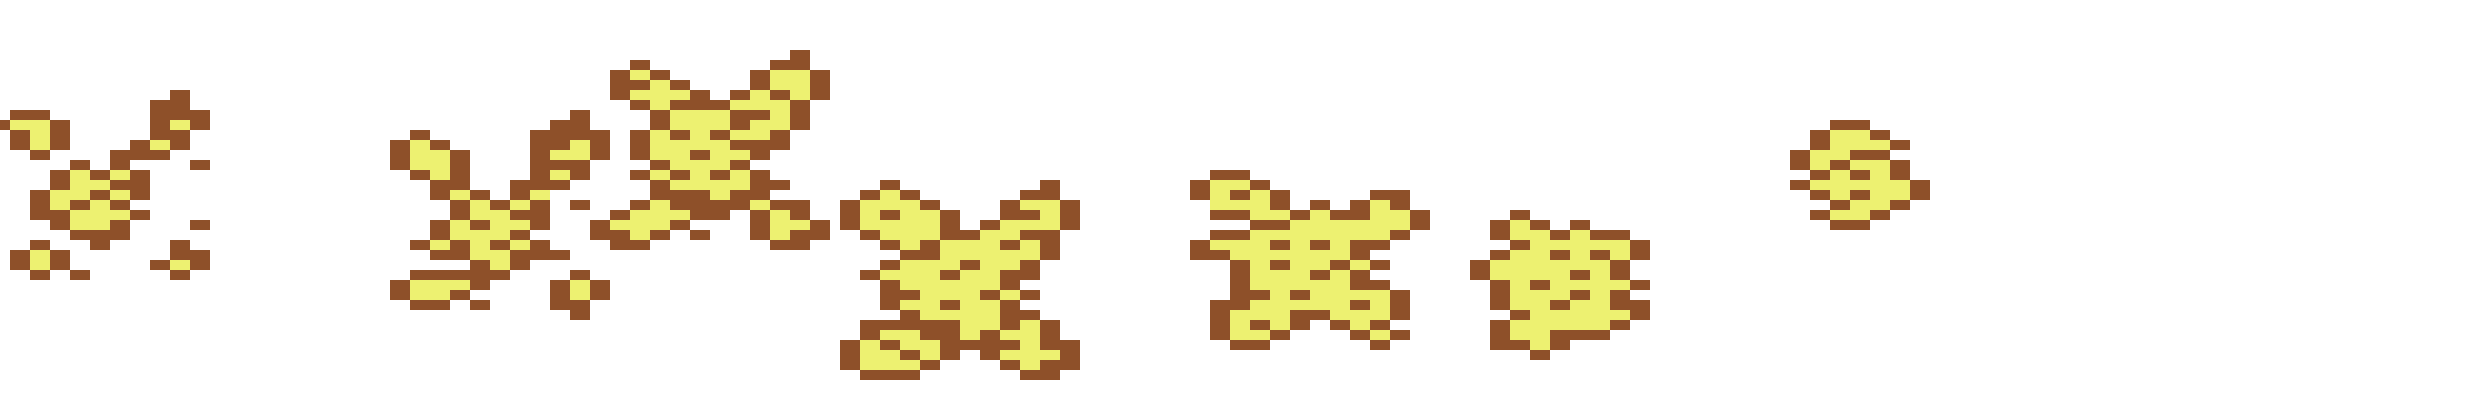
\includegraphics[height=1.6cm]{src/manta_explosion_sprites/sidebyside_explosion_7.png}%
      \hspace{0.5cm}
      \raisebox{1.2\totalheight}{
\includegraphics[height=0.4cm]{src/baydoor_sprites/arrow.png}}
      \hspace{0.3cm}
      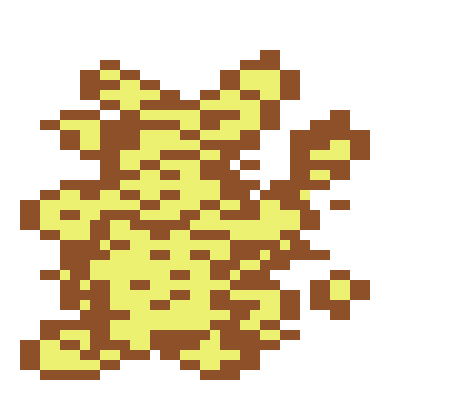
\includegraphics[height=1.6cm]{src/manta_explosion_sprites/composite_explosion_7.png}%
    \end{adjustbox}
\end{figure}
\vspace{-0.4cm}
\begin{figure}[H]
    \centering
    \begin{adjustbox}{center}
      \hspace{0.5cm}
      
\includegraphics[height=1.6cm]{src/manta_explosion_sprites/sidebyside_explosion_8.png}%
      \hspace{0.5cm}
      \raisebox{1.2\totalheight}{
\includegraphics[height=0.4cm]{src/baydoor_sprites/arrow.png}}
      \hspace{0.3cm}
      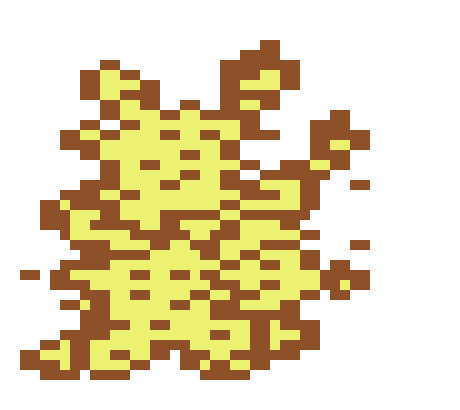
\includegraphics[height=1.6cm]{src/manta_explosion_sprites/composite_explosion_8.png}%
    \end{adjustbox}
\end{figure}
\vspace{-0.4cm}
At this point we finally have an explosion sequence active for all 8 sprites. Until now, while the
\fcode{frameCounter} in the routine opposite was still greater than \icode{-1}, we ran the
code in \fcode{AddNewMemberToSequence} to add a new member to the sequence. Notice how for
each member that we added we also calculated a random dither for its horizontal and vertical
position. It carries over this position to every subsequent frame of the animation.

From this point onwards, each iteration of the loop only has to run the code in \fcode{AnimateNextFrame}.
This segment of the routine contains a nested loop that updates each of the eight sprites to advance them to the next frame
in the 11 sprite sequence that defines a single explosion. It becomes clear as this animation advances
that the clustered burst has already reached its apex and is already en route to dissipating completely.

\fcode{MantaExplosionLoop} will keep iterating until all eight members of the sequence have been exhausted. This is
precalculated as a total of 21 frames since the \fcode{frame\-Counter} starts at 6 and \fcode{MantaExplosionLoop} will
exit when it reaches -15.

\begin{figure}[H]
    \centering
    \begin{adjustbox}{center}
      \hspace{0.5cm}
      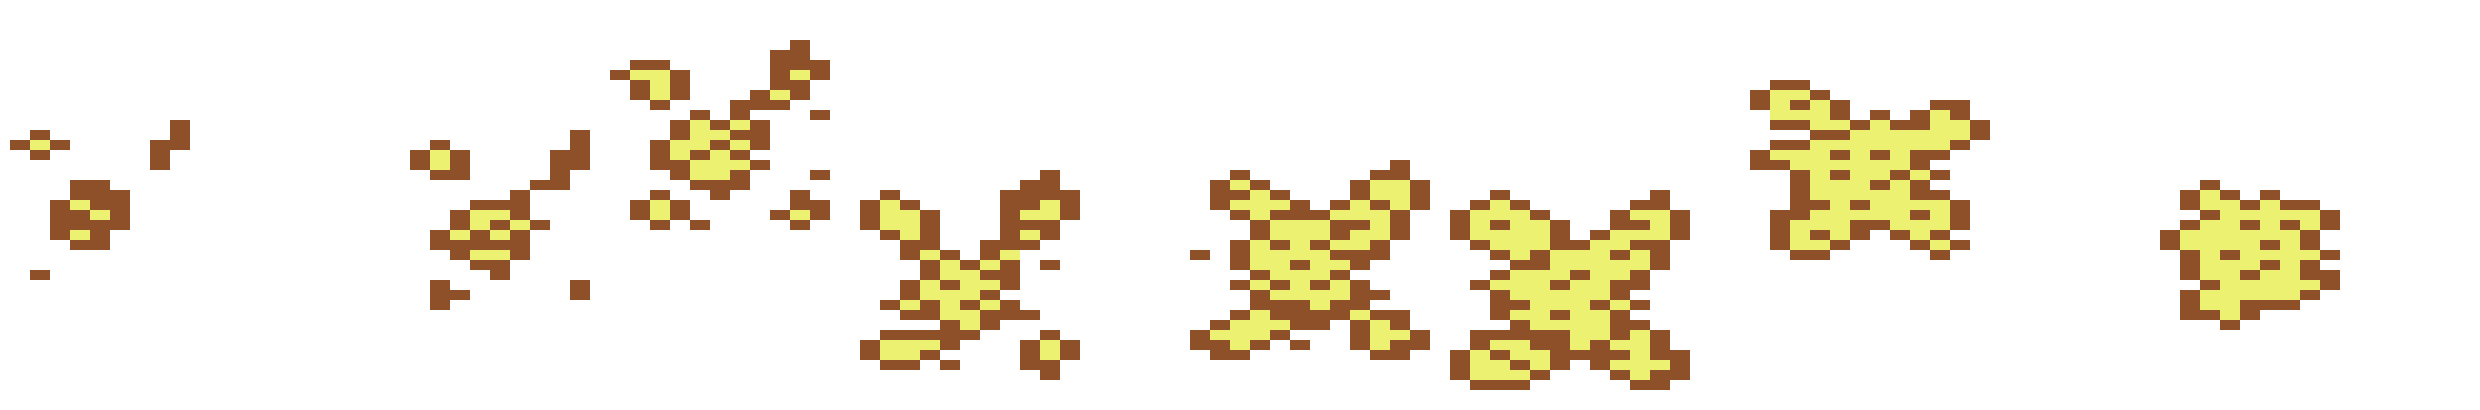
\includegraphics[height=1.6cm]{src/manta_explosion_sprites/sidebyside_explosion_9.png}%
      \hspace{0.5cm}
      \raisebox{1.2\totalheight}{
\includegraphics[height=0.4cm]{src/baydoor_sprites/arrow.png}}
      \hspace{0.3cm}
      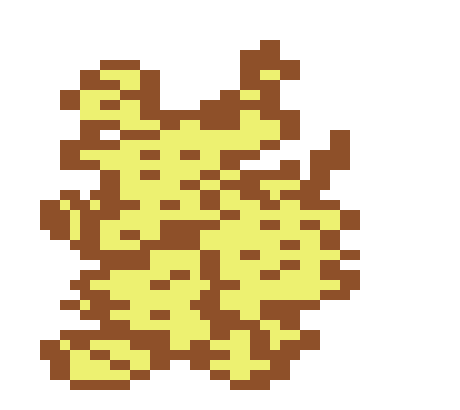
\includegraphics[height=1.6cm]{src/manta_explosion_sprites/composite_explosion_9.png}%
    \end{adjustbox}
\end{figure}
\vspace{-0.4cm}
\begin{figure}[H]
    \centering
    \begin{adjustbox}{center}
      \hspace{0.5cm}
      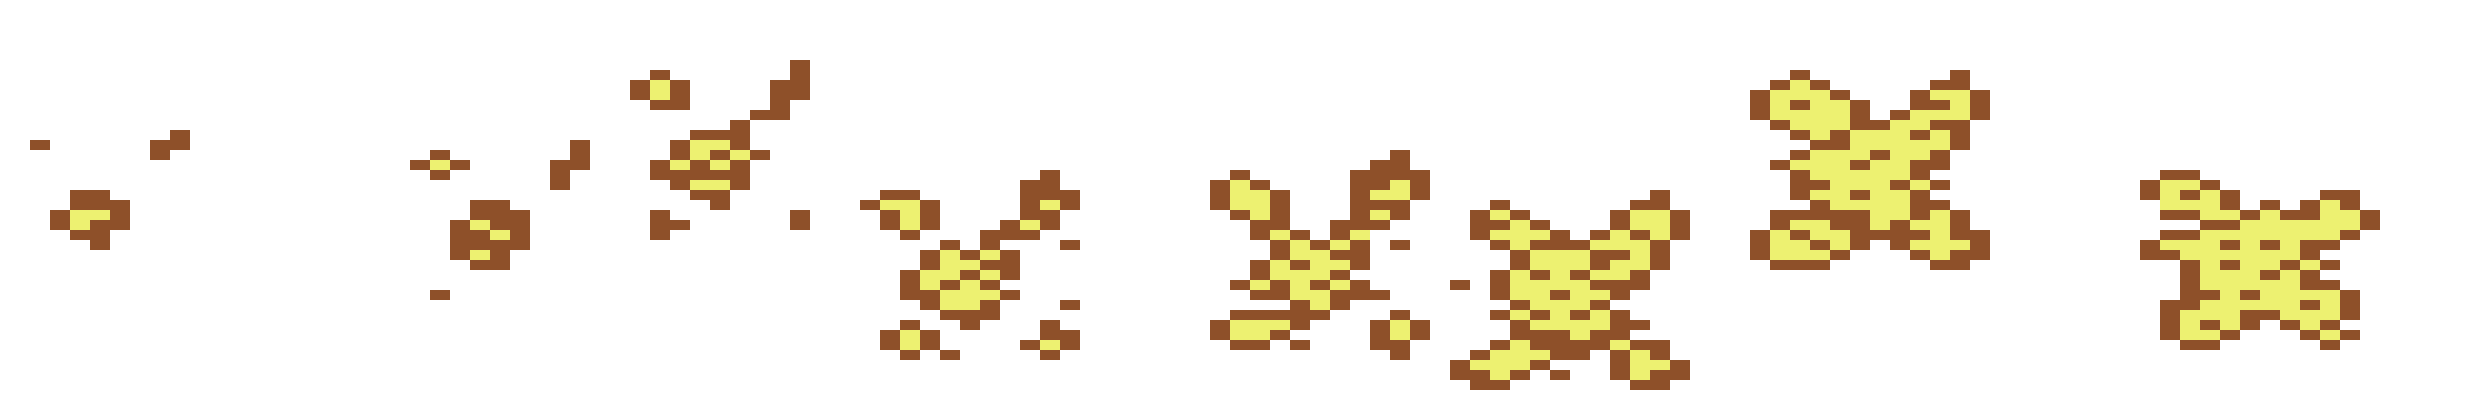
\includegraphics[height=1.6cm]{src/manta_explosion_sprites/sidebyside_explosion_10.png}%
      \hspace{0.5cm}
      \raisebox{1.2\totalheight}{
\includegraphics[height=0.4cm]{src/baydoor_sprites/arrow.png}}
      \hspace{0.3cm}
      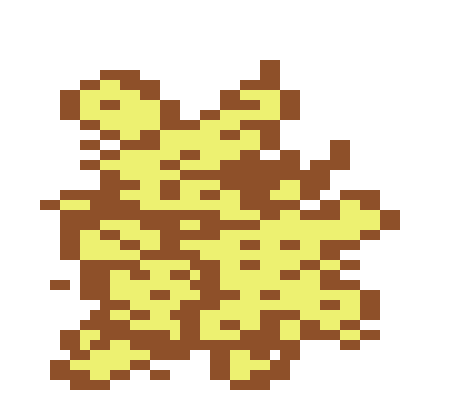
\includegraphics[height=1.6cm]{src/manta_explosion_sprites/composite_explosion_10.png}%
    \end{adjustbox}
\end{figure}
\vspace{-0.4cm}

\clearpage
\begin{lstlisting}[basicstyle=\scriptsize\ttfamily, escapechar=\%]
ExplodeTheManta
  JSR DisplayCurrentSprite    ; Display the first of the explosion sprites.

  LDA #$06
  STA frameCounter
  ; This loop fills up the sequence of 8 explosions and animates each of them
  ; through to conclusion.
MantaExplosionLoop
  LDA frameCounter            ; Get the current frame counter.
  BMI AnimateNextFrame        ; If its less than zero all eight have been added.

  ; Add a new member, there will be 8 in total - one for each sprite.
AddNewMemberToSequence
  LDA #$07                    ; Set the spriteIndex to 7 and use this..
  STA spriteIndex             ; .. to load the default initial state of..
  JSR LoadSpriteState  ; .. the explosion.

  LDA frameCounter            ; Use current frame counter (which is >= 0 and < 6)
  STA spriteIndex             ; as the spriteIndex for the new explosion sequence.

  ; Jitter the horizontal position of the explosion.
  LDA $D41B                   ; Get a random number.
  AND #$0F                    ; Make it between 0 and 15.
  SBC #$08                    ; Make it between -7 and 7.
  ADC currentSpriteXPos       ; Add the initial X position and use it to adjust..
  STA currentSpriteXPos       ; ..the final X position of the explosion.

  LDA #$30                    ; Load the sprite ref for the start of the explosion.
  STA currentSpriteValue      ; Make it the initial sprite to display.

  ; Jitter the vertical position of the explosion.
  LDA $D41B                   ; Get a random number.
  AND #$0F                    ; Make it between 0 and 15.
  SBC #$08                    ; Make it between -7 and 7.
  ADC currentSpriteYPos       ; Add the initial X position and use it to adjust..
  STA currentSpriteYPos       ; ..the final X position of the explosion.

  JSR UpdateSpriteAndDisplay  ; Display the new member of the sequence.

  ; Do the animation for all 8 sprites in the sequence, skipping any that have
  ; not been activated yet.
AnimateNextFrame
  LDA #$07                    ; Set spriteIndex to 7 so that we decrement 
  STA spriteIndex             ; by one until we reach zero.
AdvanceEachSpriteByAFrame                                                         
  JSR LoadSpriteState         ; Get the current state of this member.
  INC currentSpriteValue      ; Increment it sprite to the next frame.
  LDA currentSpriteValue      ; Check the new frame.. 
  CMP #$3B                    ; If there are more frames to do for this member..  
  BCC NextExplosionFrame      ; .. then go to the next member, otherwise.. 
  LDA #$00                    ; Stop displaying this sprite because..
  STA currentSpriteEnabled    ; .. it has finished.
NextExplosionFrame
  JSR UpdateSpriteAndDisplay  ; Display the updated member of the sequence.
  DEC spriteIndex             ; Go to the next member.
  BPL AdvanceEachSpriteByAFrame ; Loop until we reach the last one.

  ; Keep looping until all eight sprites have completed a full explosion.
  DEC frameCounter            ; Decrement the Frame counter.
  LDA frameCounter            ; Get the new value of the frame counter.
  CMP #-15                    ; Has it reached -15 yet?
  BEQ ExitMantaExplosion      ; If so, we're done..
  JMP MantaExplosionLoop      ; .. otherwise keep looping.
\end{lstlisting}

\begin{figure}[H]
    \centering
    \begin{adjustbox}{center}
      \hspace{0.5cm}
      
\includegraphics[height=1.6cm]{src/manta_explosion_sprites/sidebyside_explosion_11.png}%
      \hspace{0.5cm}
      \raisebox{1.2\totalheight}{
\includegraphics[height=0.4cm]{src/baydoor_sprites/arrow.png}}
      \hspace{0.3cm}
      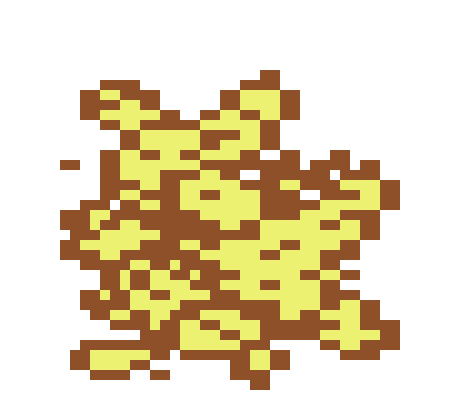
\includegraphics[height=1.6cm]{src/manta_explosion_sprites/composite_explosion_11.png}%
    \end{adjustbox}
\end{figure}
\vspace{-0.4cm}

Within three frames the first member of the sequence is exhausted. The bulk of the explosion 
does not look much diminished. But with each successive frame, another sprite ends its contribution
to the sequence - the blast starts its inevitable path to total evaporation.
\begin{figure}[H]
    \centering
    \begin{adjustbox}{center}
      \hspace{0.5cm}
      
\includegraphics[height=1.6cm]{src/manta_explosion_sprites/sidebyside_explosion_12.png}%
      \hspace{0.5cm}
      \raisebox{1.2\totalheight}{
\includegraphics[height=0.4cm]{src/baydoor_sprites/arrow.png}}
      \hspace{0.3cm}
      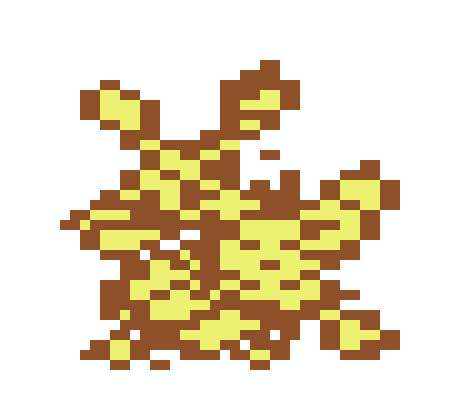
\includegraphics[height=1.6cm]{src/manta_explosion_sprites/composite_explosion_12.png}%
    \end{adjustbox}
\end{figure}
\vspace{-0.4cm}
\begin{figure}[H]
    \centering
    \begin{adjustbox}{center}
      \hspace{0.5cm}
      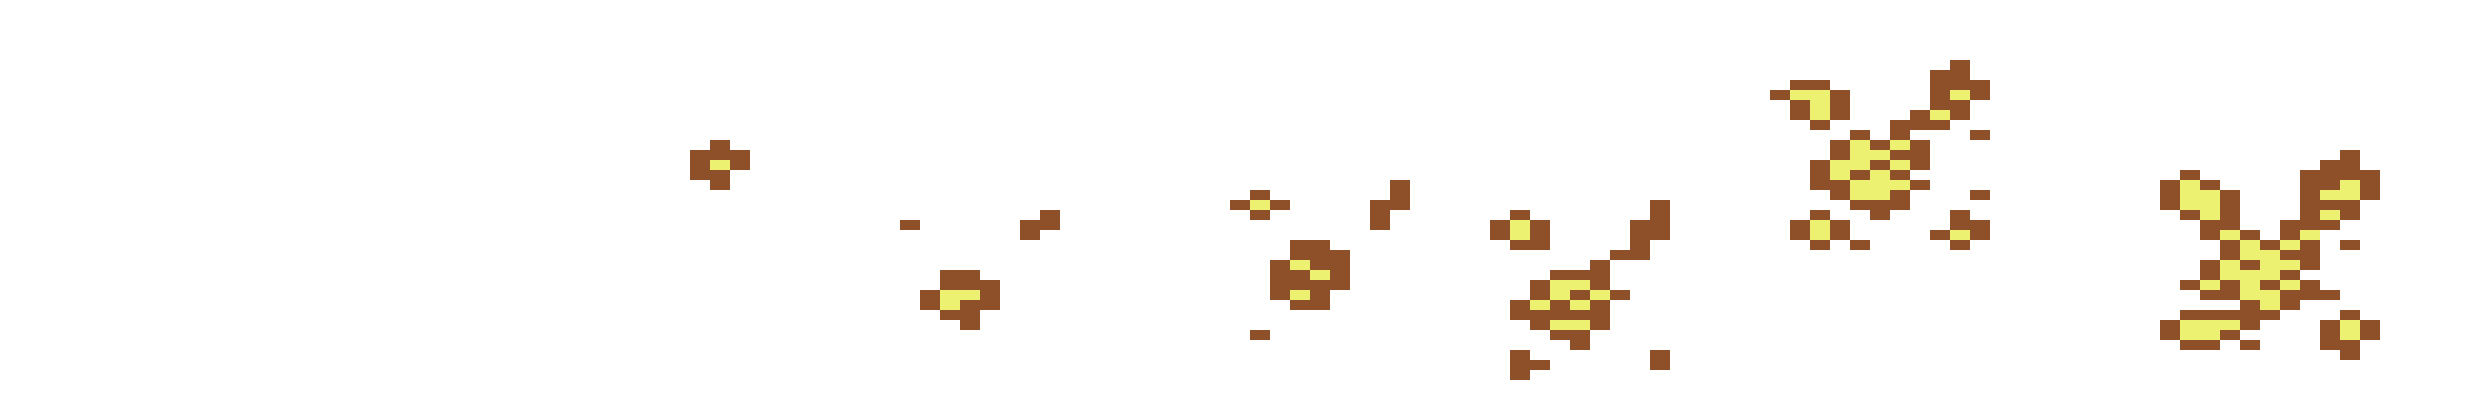
\includegraphics[height=1.6cm]{src/manta_explosion_sprites/sidebyside_explosion_13.png}%
      \hspace{0.5cm}
      \raisebox{1.2\totalheight}{
\includegraphics[height=0.4cm]{src/baydoor_sprites/arrow.png}}
      \hspace{0.3cm}
      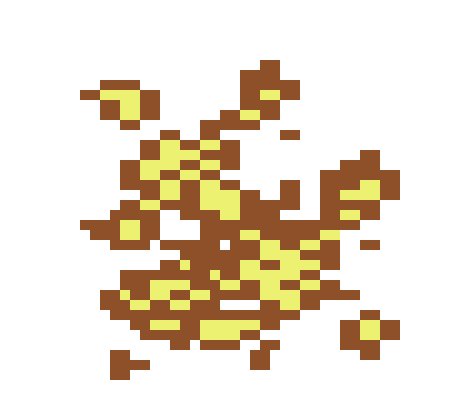
\includegraphics[height=1.6cm]{src/manta_explosion_sprites/composite_explosion_13.png}%
    \end{adjustbox}
\end{figure}
\vspace{-0.4cm}
\begin{figure}[H]
    \centering
    \begin{adjustbox}{center}
      \hspace{0.5cm}
      
\includegraphics[height=1.6cm]{src/manta_explosion_sprites/sidebyside_explosion_14.png}%
      \hspace{0.5cm}
      \raisebox{1.2\totalheight}{
\includegraphics[height=0.4cm]{src/baydoor_sprites/arrow.png}}
      \hspace{0.3cm}
      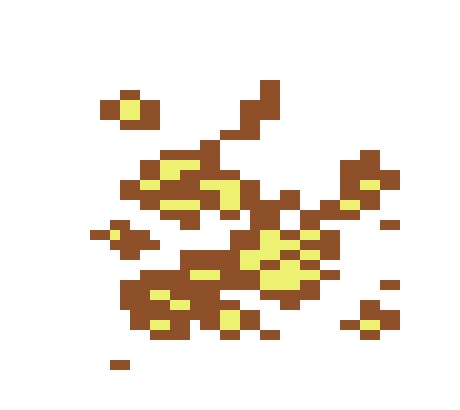
\includegraphics[height=1.6cm]{src/manta_explosion_sprites/composite_explosion_14.png}%
    \end{adjustbox}
\end{figure}
\vspace{-0.4cm}
\begin{figure}[H]
    \centering
    \begin{adjustbox}{center}
      \hspace{0.5cm}
      
\includegraphics[height=1.6cm]{src/manta_explosion_sprites/sidebyside_explosion_15.png}%
      \hspace{0.5cm}
      \raisebox{1.2\totalheight}{
\includegraphics[height=0.4cm]{src/baydoor_sprites/arrow.png}}
      \hspace{0.3cm}
      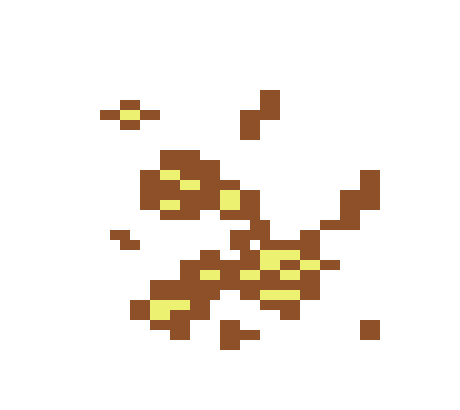
\includegraphics[height=1.6cm]{src/manta_explosion_sprites/composite_explosion_15.png}%
    \end{adjustbox}
\end{figure}
\vspace{-0.4cm}
\begin{figure}[H]
    \centering
    \begin{adjustbox}{center}
      \hspace{0.5cm}
      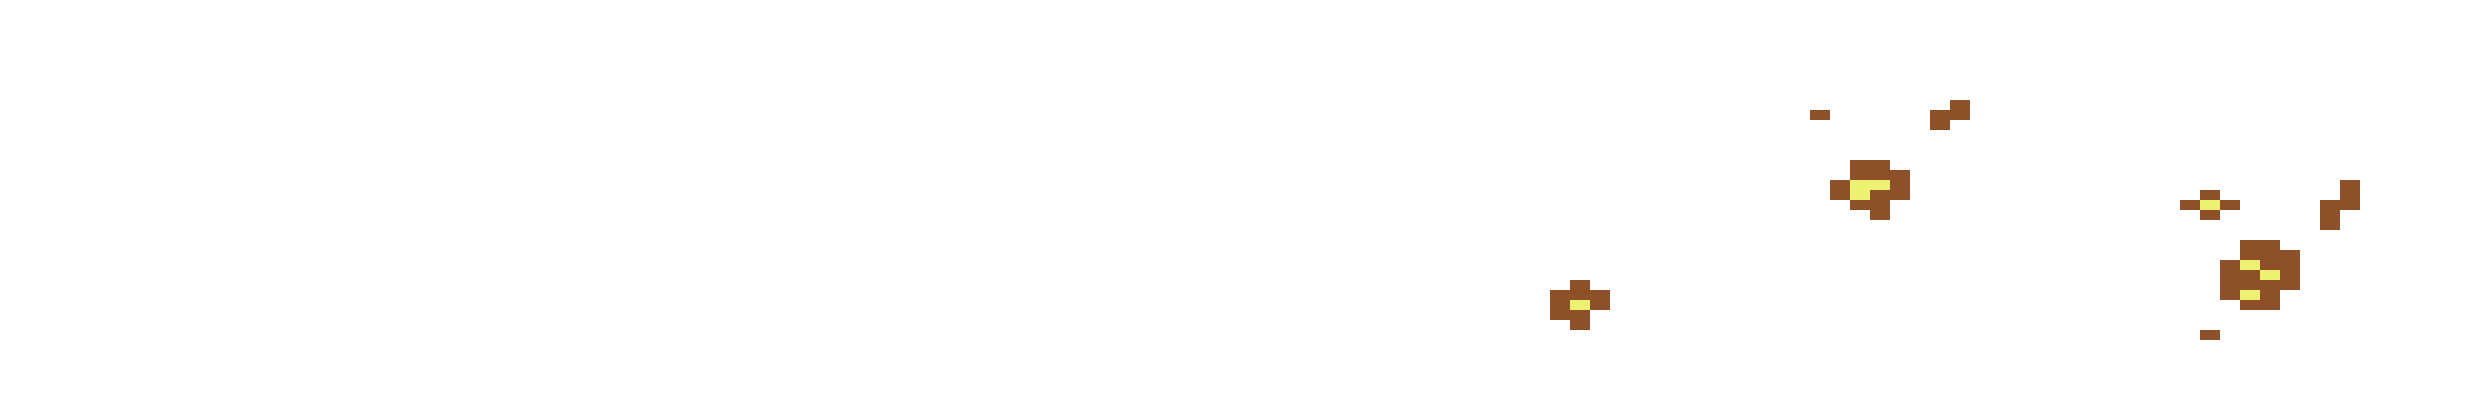
\includegraphics[height=1.6cm]{src/manta_explosion_sprites/sidebyside_explosion_16.png}%
      \hspace{0.5cm}
      \raisebox{1.2\totalheight}{
\includegraphics[height=0.4cm]{src/baydoor_sprites/arrow.png}}
      \hspace{0.3cm}
      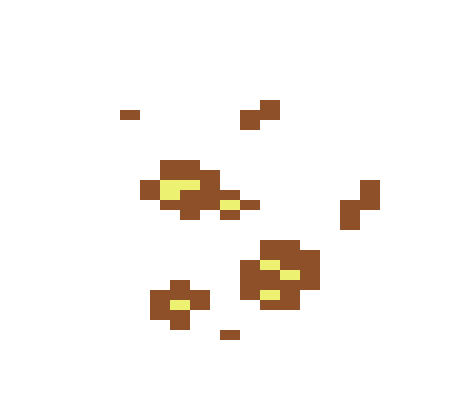
\includegraphics[height=1.6cm]{src/manta_explosion_sprites/composite_explosion_16.png}%
    \end{adjustbox}
\end{figure}
\vspace{-0.4cm}
\begin{figure}[H]
    \centering
    \begin{adjustbox}{center}
      \hspace{0.5cm}
      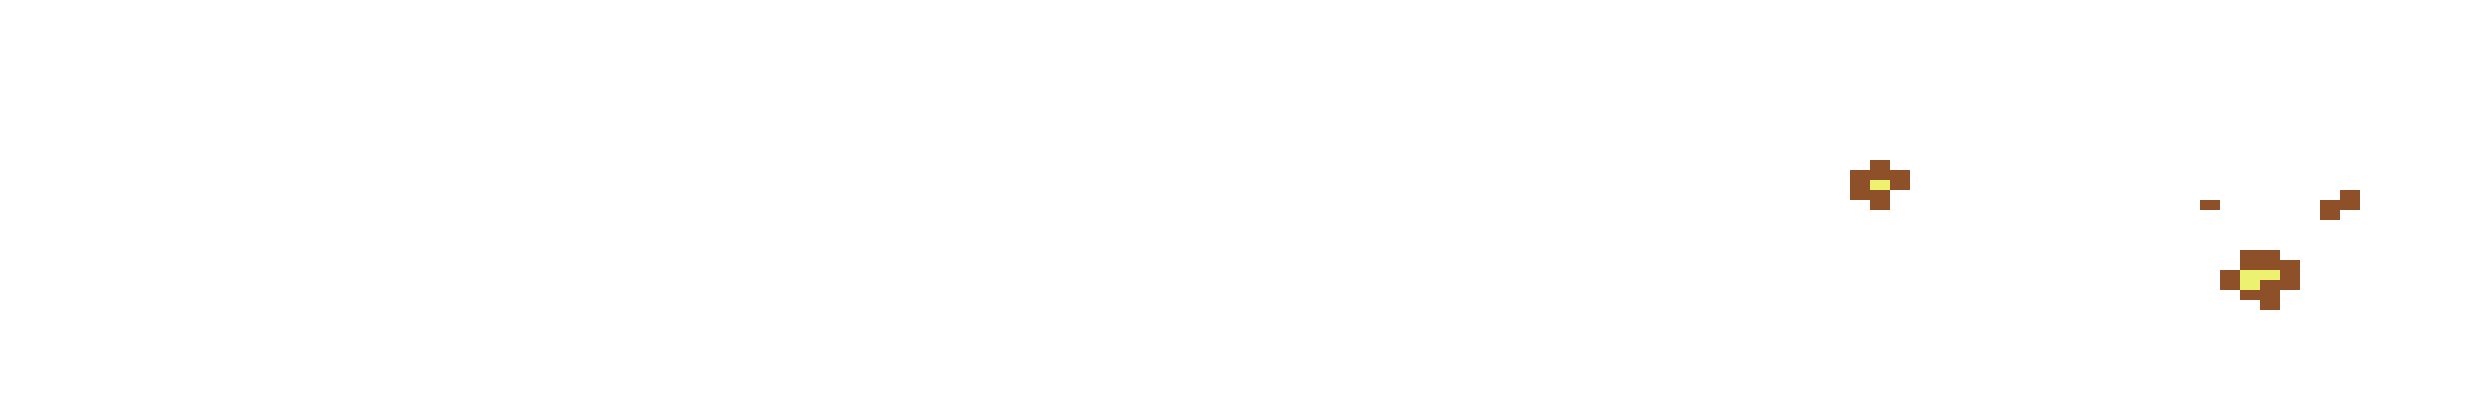
\includegraphics[height=1.6cm]{src/manta_explosion_sprites/sidebyside_explosion_17.png}%
      \hspace{0.5cm}
      \raisebox{1.2\totalheight}{
\includegraphics[height=0.4cm]{src/baydoor_sprites/arrow.png}}
      \hspace{0.3cm}
      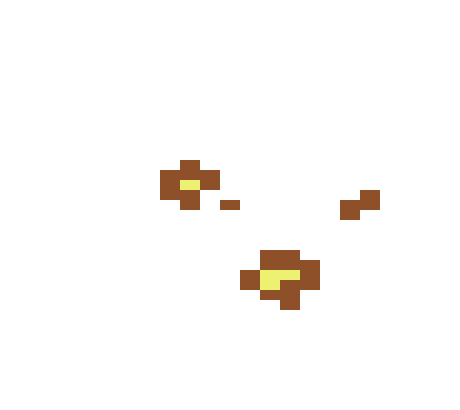
\includegraphics[height=1.6cm]{src/manta_explosion_sprites/composite_explosion_17.png}%
    \end{adjustbox}
\end{figure}
\vspace{-0.4cm}
\begin{figure}[H]
    \centering
    \begin{adjustbox}{center}
      \hspace{0.5cm}
      
\includegraphics[height=1.6cm]{src/manta_explosion_sprites/sidebyside_explosion_18.png}%
      \hspace{0.5cm}
      \raisebox{1.2\totalheight}{
\includegraphics[height=0.4cm]{src/baydoor_sprites/arrow.png}}
      \hspace{0.3cm}
      
\includegraphics[height=1.6cm]{src/manta_explosion_sprites/composite_explosion_18.png}%
    \end{adjustbox}
\end{figure}
\vspace{-0.4cm}

